\documentclass{bookest}

\usepackage{hyperref}
\usepackage{amsmath}
\usepackage{amssymb}
\usepackage{amsthm}
\usepackage{graphics}
\usepackage{graphicx}
\usepackage{floatrow}
\usepackage{tikz}
\usepackage{color}
\usepackage{algorithm}
\usepackage{algorithmicx}
\usepackage{algpseudocode}
\usepackage{caption}
\usepackage{subcaption}



\newcommand{\reals}{\mathbb{R}}
\newcommand{\integers}{\mathbb{Z}}
\newcommand{\symm}{\mathbb{S}}  % symmetric matrices

\newcommand{\rank}{\mathop{\bf rank}}
\newcommand{\tr}{\mathop{\bf tr}}
\newcommand{\diag}{\mathop{\bf diag}}
\renewcommand{\rank}{\mathop{\bf rank}}
\newcommand{\conv}{\mathop{\bf conv}}
\newcommand{\spans}{\mathop{\bf span}}
\newcommand{\nulls}{\mathop{\bf null}}
\newcommand{\clo}{\mathop{\bf clo}}

\renewcommand{\det}{\mathop{\bf det}}
\newcommand{\proj}{\mathop{\bf proj}}
\newcommand{\argmin}{\mathop{\rm argmin}}
\newcommand{\argmax}{\mathop{\rm argmax}}
\newcommand{\epi}{\mathop{\bf epi}} % epigraph
\newcommand{\dom}{\mathop{\bf dom}} % domain
\newcommand{\intr}{\mathop{\bf int}}
\newcommand{\bou}{\mathop{\bf bou}}

\newcommand{\mini}{\mathop{\text{min.~}}}
\newcommand{\maxi}{\mathop{\text{max.~}}}
\newcommand{\minf}{\mathop{\text{minimize~}}}
\newcommand{\maxf}{\mathop{\text{maximize~}}}
\newcommand{\st}{\mathop{\text{s.t.:~}}}
\newcommand{\stf}{\mathop{\text{subject to:~}}}

\newcommand{\braces}[1]{\left\{ #1 \right \}}
\newcommand{\brackets}[1]{\left[ #1 \right]}
\newcommand{\floor}[1]{\lfloor #1 \rfloor}
\newcommand{\ceil}[1]{\lceil #1 \rceil}

\newcommand{\lb}{\linebreak}

\newtheorem{theorem}{Theorem}
\newtheorem*{theorem*}{Theorem}
\newtheorem{proposition}[theorem]{Proposition}
\newtheorem*{remark}{Remark}
\newtheorem{assumption}[theorem]{Assumption}
\newtheorem{definition}[theorem]{Definition}
\newtheorem{lemma}[theorem]{Lemma}
\newtheorem{corollary}[theorem]{Corollary}




\parindent 1cm
\parskip 0.2cm
\topmargin 0.2cm
\oddsidemargin 1cm
\evensidemargin 0.5cm
\textwidth 15cm
\textheight 21cm


\title{Optimisation notes}

\begin{document}
	\maketitle

	\tableofcontents
	
	\part{Linear optimisation}
	
	\chapter{Introduction}
	\section{What is optimisation?}

An optimisation is one of these words that has many meanings, depending on the context you take as a reference. In the context of this course, optimisation refers to \emph{mathematical optimisation}, which is a discipline of applied mathematics.

In mathematical optimisation, we build upon concepts and techniques from calculus, analysis, linear algebra, and other domains of mathematics to develop methods that allow us finding values for variables within a given domain that maximise (or minimise) the value of a function. In specific, we are trying to solve the following general problem:
%
\begin{align}
    \mini & f(x) \label{eq:opt_prob} \\
    \text{s.t.}   &x \in X. \nonumber
\end{align}
%
%where $x \in \reals^n$ is a vector of $n$ \emph{variables}, $f:\mathbb{R}^n \mapsto \reals$ is a \emph{function} to be optimised (minimised) and $X \subseteq \reals^n$ is a \emph{domain} containing acceptable values for $x$.

In a general sense, these problems can be solved by employing the following strategy:
%
\begin{enumerate}
    \item Analysing properties of functions under specific domains and deriving the conditions that must be satisfied such that a point $x$ is a candidate optimal point.
    \item Applying numerical methods that iteratively searches for points satisfying these conditions. 
\end{enumerate}
%
This idea is central in several domains of knowledge, and very often are defined under area-specific nomenclature. Fields such as economics, engineering, statistics, machine learning and, perhaps more broadly, operations research, are intensive users and developers of optimisation theory and applications. 

\subsection{Mathematical programming and optimisation}

Operations research and mathematical optimisation are somewhat intertwined, as they both were born around a similar circumstance. %(Include something on the history of OR)

I like to separate \emph{mathematical programming} from (mathematical) \emph{optimisation}. Mathematical programming is a modelling paradigm, in which we rely on (very powerful, I might add) analogies to model \emph{real-world} problems. In that, we look at a given decision problem considering that
%
\begin{itemize}
    \item \emph{variables} represent \emph{decisions}, as in a business decision or a course of action. Examples include setting the parameter of (e.g., prediction) model, production systems layouts, geometries of structures, topologies of networks, and so forth; 
    \item \emph{domain} represents business rules or \emph{constraints}, representing logic relations, design or engineering limitations, requirements, and such; 
    \item function is an \emph{objective function} that provides a measure of solution quality.  
\end{itemize}
%    
With these in mind, we can represent the decision problem as a \emph{mathematical programming model} of the form of \eqref{eq:opt_prob} that can be solved using \emph{optimisation} methods. From now on, we will refer to this specific class of models as mathematical optimisation models, or optimisation models for short. We will also use the term to \emph{solve the problem} to refer to the task of finding optimal solutions to optimisation models.

This course is mostly focused on the optimisation techniques employed to find optimal solutions for these models. As we will see, depending on the nature of the functions $f$ and $g$ that are used to formulate the model, some methods might be more or less appropriate. Further complicating the issue, for models of a given nature, there might be alternative algorithms that can be employed and with no generalised consense whether one method is generally better performing than another.

\subsection{Types of mathematical optimisation models}

In general, the simpler the assumptions on the parts forming the optimisation model, the more efficient are the methods to solve such problems. 

Let us define some additional notation that we will use from now on. Consider a model in the general form
%
\begin{align*}
	\mini & f(x) \\
	\st   & g_i(x) \leq 0, i = 1, \dots, m \\
	      & h_i(x) = 0, i = 1, \dots, l \\
	      & x \in X,  
\end{align*}
%
where $f: \reals^n \mapsto \reals$ is the objective function, $g:\reals^m \mapsto \reals^m$ is a collection of $m$ inequality constraints and $h: \reals^n \mapsto \reals^l$ is a collection of $l$ equality constraints.

{\bf Remark:} in fact, every inequality constraint can be represented by an equality constraint by making $h_i(x) = g_i(x) + x_{n+1}$ and augmenting the decision variable vector $x \in \reals^n$ to include the slack variable $x_{n+1}$. However, since these constraints are of very different nature, we will explicitly represent both whenever necessary.

The most general types of models are the following. We also use this as an opportunity to define some (admittedly confusing) nomenclature from the field of operations research that we will be using in these notes.
%
\begin{enumerate}
    \item \emph{Unconstrained models:} in these, the set $X = \reals^n$ and $m=l=0$. These are prominent in, e.g., machine learning and statistics applications, where $f$ represents a measure of model fitness or prediction error.  
    \item \emph{Linear programming (LP):} presumes linear objective function. $f(x) = c^\top x$ and constraints $g$ and $h$ affine, i.e., of the form $a_i^\top x - b_i$, with $a_i \in \reals^n$ and $b \in \reals$. Normally, $X = \braces{x \in \reals^n \mid x_j \geq 0, j = 1,\dots, n}$ enforce that decision variables are constrained to be the nonnegative orthant.
    \item \emph{Nonlinear programming (NLP):} some or all of the functions $f$, $g$, and $h$ are nonlinear.
    \item \emph{Mixed-integer (linear) programming (MIP):} consists of an LP in which some (or all) of the variables are constrained to be integers. In other words, $X \subseteq \reals^k \times \integers^{n-k}$. Very frequently, the integer variables are binary terms, i.e., $x_i \in \braces {0,1}$, for $i = 1,\dots, n-k$ and are meant to represent true-or-false or yes-or-no conditions.
    \item \emph{Mixed-integer nonlinear programming (MINLP):} are the intersection of MIPs and NLPs.  
\end{enumerate}

{\bf Remark:} notice that we use the vector notation $c^\top x = \sum_{j \in J} c_j x_j$, with $J = \braces{1,\dots,N}$. This is just a convenience for keeping the notation compact. 


\section{Linear programming applications}

We will consider now a few examples of liner programming models with somewhat general structure. Many of these examples have features that can be combined into more general models.


\subsection{Resource allocation}

Most linear programming (LP) problems, can be interpreted as a \emph{resource allocation} problem. In that, we are interested in defining an optimal allocation of resources (i.e., a plan) that maximises return or minimise costs and satisfy allocation rules. 

Specifically, let $I = \braces{1, \dots, i, \dots, M}$ by a set of resources that can be combined to produce products in the set $J = \braces{1, \dots, j, \dots, N}$. Assume that we are given a return per unit of product $c_j$, $\forall j\in J$ and a list of $a_{ij}$, $\forall i \in I, \forall j \in J$ describing which and how much of the resources $i \in I$ are required for making product $j \in J$. Assume that the availability of resource $b_i$, $\forall i\in I$, is known. 

Our objective is to define the amounts $x_j$ representing the production of $j \in J$. We would like to define those in a way that we optimise the resource allocation plan quality (in our case, maximise return from the production quantities $x_j$) while making sure the amount produced do not exceed the availability of resources. For that, we need to define: 

The \emph{objective function}, which measures the \emph{quality} of a production plan. In this case, the total return for a given plan is given by:
%
\begin{equation*}
	\maxi \sum_{j \in J}c_jx_j \Rightarrow c^\top x,
\end{equation*}
%
where $c = [c_1, \dots, c_{N}]^\top$ and $x = [x_1, \dots, x_{N}]^\top$ are $n$-sized vectors.


Next, we need to define \emph{constraints} that state the conditions for a plan to be \emph{valid}. In this context, a valid plan is a plan that does not utilise more than the amount of resources $b_i$, $\forall i \in I$ available. This can be expressed as the collection (one for each $i \in I$) of linear inequalities
%
\begin{equation*}
	\st \sum_{j \in J} a_{ij}x_j \leq b_i, \forall i \in I	\Rightarrow	Ax \leq b,
\end{equation*}
%
where $a_{ij}$ are the components of the $M \times N$ matrix $A$ and $b = [b_1,\dots, b_M]^\top$. Furthermore, we also must require that $x_i \geq 0, \forall i \in I$.                                                                                                         

Combining the above, we obtain the generic formulation that will be used throughout this text to represent linear programming models:
%
\begin{align}
	\maxi & c^\top x  \label{p1c1:eq:LP_objective} \\
	\st   & Ax \leq b \label{p1c1:eq:LP_constraint} \\
		  & x \geq 0. \label{p1c1:eq:LP_domain}
\end{align}
%

\subsubsection{Illustrative example: the paint factory problem}
 
Let us work on a more specific example, that will be useful for illustrating some important concepts related to the geometry of linear programming problems.

A paint factory produces \emph{exterior} and \emph{interior paint} from raw materials \emph{M1} and \emph{M2}. The \emph{maximum demand} for interior paint is 2 tons/day. Moreover, the amount of interior paint produced \emph{cannot exceed} that of exterior paint by more than 1 ton/day. 

Our goal is to determine optimal paint production plan. Table \ref{p1c1:tab:paint_factory_problem_data} summarises the data to be considered. Notice the constraint that must be imposed to represent the daily availability of paint.

\begin{table}[h]
	\begin{tabular}{rccc} \hline
	&\multicolumn{2}{c}{material (ton)/paint (ton)}\\ \hline
	& exterior paint & interior paint & daily availability (ton)\\ \hline
	material M1 & 6 & 4 & 24\\
	material M2 & 1 & 2 & 6\\ \hline
	profit (\$1000 /ton) & 5 & 4\\ \hline
	\end{tabular}
	\caption{Paint factory problem data} \label{p1c1:tab:paint_factory_problem_data}
\end{table}

Notice that the paint factory problem is an example of a resource allocation problem. Perhaps one aspect that is somewhat dissimilar is the constraint representing the production rules regarding the relative amounts of interior and exterior paint. Notice however, that this type of constraint also has the same format as the more straightforward resource allocation constraints.  

Let $x_1$ be amount produced of exterior paints (in tons) and $x_2$ the amount of interior paints. The complete model that optimises the daily production plan of the paint factory is:
%
\begin{flalign}
	\maxi z = \ & 5x_1 + 4x_2 \label{p1c1:eq:constM1}\\
	\st & 6x_1 + 4x_2 \leq 24 \label{p1c1:eq:constM2}\\
	& x_1 + 2x_2 \leq 6 \\
	& x_2 - x_1 \leq  1 \\
	& x_2 \leq 2 \\
	& x_1, x_2 \geq 0
\end{flalign}
%
Notice that paint factory model can also be \emph{compactly represented} as in \eqref{p1c1:eq:LP_objective}--\eqref{p1c1:eq:LP_domain}, where
%
\begin{equation*}
	c = [5, 4]^\top, \ x = [x_1, x_2]^\top, \ A = \begin{bmatrix} 6 & 4 \\ 1 & 2 \\ -1 & 1 \\0 & 1 \end{bmatrix}, \text{ and } b = [24, 6, 1, 2]^\top.	
\end{equation*}
%


\subsection{Transportation problem}

Another important class of linear programming problems are those known as transportation problems. These problems are often model using the abstraction of graphs, since they consider a network of nodes and arcs through which some flow must be optimised. Transportation problems have several important characteristics that can be exploit to design specialised algorithms, the so-called \emph{transportation simplex} method. Although we will not discuss these methods in this text, the simplex method (and its variant dual simplex) will be in the centre of our developments later on. Also, modern solvers have more and more relegate transport simplex methods in their development, as dual simplex has consistently shown to perform similarly in the context of transportation problems, despite being a far more general method. 

The problem can be summarised as follows. We would like to plan production and distribution of a certain product, taking into account that the transportation cost is known (e.g., proportional to distance travelled), the factories (or source nodes) have a capacity limit and the clients (or demand nodes) have known demands. Figure \ref{p1c1:fig1:transport_network} illustrate a small network with two factories, located in San Diego and Seattle, and three demand points, located in New York, Chicago, and Miami. Table \ref{p1c1:tab:transport_problem_data} presents the data related to the problem. 
%
\begin{figure}[h]
	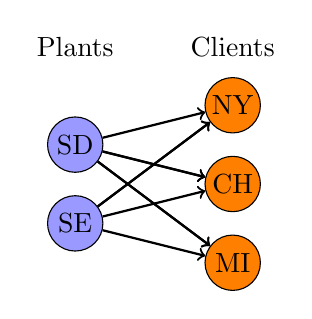
\begin{tikzpicture}[scale=1,
		node/.style={circle, fill=blue!40, draw, minimum size=2em, inner sep=1pt},
		node2/.style={circle, fill=orange, draw, minimum size=2em, inner sep=1pt}] 
    	\node[above] at (0, 3.5) {Plants};                                                                                  
    	\node[above] at (2, 3.5) {Clients};
	    \node[node] (1) at (0, 1.5) {SE};
	    \node[node] (2) at (0, 2.5) {SD};
	    \node[node2] (3) at (2, 3) {NY};
	    \node[node2] (4) at (2, 2) {CH};
	    \node[node2] (5) at (2, 1) {MI};
	    \foreach \x in {1,...,2} {
	       \foreach \y in {3,...,5} {
	          \draw[->, thick] (\x) -- (\y);
	          }}      
	    \draw[->, thick] (1) -- (3);
	    \draw[->, thick] (2) -- (4);
	    \draw[->, thick] (2) -- (5);                            
	\end{tikzpicture}
	\caption{Schematic illustration of a network with two source nodes and three demand nodes} \label{p1c1:fig1:transport_network}    
\end{figure}
%
\begin{table}
	\begin{tabular}{r|ccc|c}
    	& & {\it Clients} &\\\hline
    	{\it Factory} & NY & Chicago & Miami & Capacity \\\hline
    	Seattle & 2.5      & 1.7    & 1.8   & 350 \\
    	San Diego & 3.5 & 1.8 & 1.4 & 600 \\\hline
    	Demands & 325 & 300 & 275 & - \\\hline
	\end{tabular}
	\caption{Problem data: unit transportation costs, demands and capacities} \label{p1c1:tab:transport_problem_data}
\end{table}

To formulate a linear programming model representing the transportation problem, let $i \in I = \{\text{Seattle}, \text{San Diego}\}$ be the index set representing factories. Similarly, let $j \in J = \{\text{New York}, \text{Chicago}, \text{Miami}\}$.

The decisions in this case are represented by $x_{ij}$ be the amount produced in factory $i$ and sent to client $j$. Such a distribution plan can then be assessed by its total transportation cost, which is given by
%
$$ 
\mini z = 2.5x_{11} + 1.7x_{12} + 1.8x_{13} + 3.5x_{21} + 1.9x_{22} + 1.4x_{23}.
$$
%
The total transportation cost can be more generally represented as
%
$$
\mini z = \sum_{i \in I}\sum_{j \in J}c_{ij}x_{ij}
$$
%
where $c_{ij}$ is the unit transportation cost from $i$ to $j$.
%
The problem has two types of constraints that must be observed, relating to the supply capacity and demand requirements. These can be stated as the following linear constraints
%
\begin{align*}
	& x_{11} + x_{12} + x_{13} \leq 350 \text{ (capacity limit in Seattle)}\\
	& x_{21} + x_{22} + x_{23} \leq 600 \text{ (capacity limit in San Diego)}\\
	& x_{11} + x_{21} \geq 325 \text{ (demand in New York)}\\
	& x_{12} + x_{22} \geq 300 \text{ (demand in Chicago)}\\
	& x_{13} + x_{23} \geq 275 \text{ (demand in Miami)}.
\end{align*}
%
These constraints can be expressed in the more compact form
%
\begin{align}
	& \sum_{j \in J} x_{ij} \leq C_i, \forall i  \label{p1c1:eq:transportation_constraint_supply}\\
	& \sum_{i \in I} x_{ij} \geq D_j, \forall j, \label{p1c1:eq:transportation_constraint_demand}
\end{align}

where $C_i$ is the production capacity of factory $i$ and $D_j$ is the demand of client $j$. Notice that the terms on the lefthand side in \eqref{p1c1:eq:transportation_constraint_supply} accounts for the total production in each of the source nodes $i \in I$. Analogously, in constraint \eqref{p1c1:eq:transportation_constraint_demand}, the term on the left accounts for the total of the demand satisfied at the demand nodes $j \in J$. Using an optimality argument stating that any solution for which, for any $j \in J$, $\sum_{i \in I} x_{ij} > D_j$ can be improved by making $\sum_{i \in I} x_{ij} = D_j$. This show that his constraint under these conditions will always be satisfied as an equality constraint instead, and could be replaced like such. 

The complete transportation model for the example above can be stated as 
%
\begin{align*}
	\mini z = \ &2.5x_{11} + 1.7x_{12} + 1.8x_{13} + 3.5x_{21} + 1.9x_{22} + 1.4x_{23} \\
	\st & x_{11} + x_{12} + x_{13} \leq 350, \ 
	x_{21} + x_{22} + x_{23} \leq 600\\
	& x_{11} + x_{21} \geq 325, \ x_{12} + x_{22} \geq 300, \ x_{13} + x_{23} \geq 275\\
	& x_{11}, \dots, x_{23} \geq 0.
\end{align*}
%

Or, more compactly, in the so called \emph{algebraic (or symbolic) form}
%
\begin{align*}
	\mini z = \ &\sum_{i \in I}\sum_{j \in J}c_{ij}x_{ij}\\
	\st & \sum_{j \in J} x_{ij} \leq C_i, \forall i\\
	& \sum_{i \in I} x_{ij} \geq D_j, \forall j\\
	&x_{ij} \geq 0, \forall i \in I, \forall j \in J.
\end{align*}
%
One interesting aspect to notice regarding algebraic forms is that they allow to represent the main structure of the model while being independent of the instance being considered. For example, regardless of whether the instance would have 5 or 50 nodes, the algebraic formulation is the same, allowing for detaching the problem instance (in our case the 5 node network) from the model itself. Moreover, most computational tools for mathematical programming modelling (hereinafter referred to simply as modelling - like JuMP) requires the user to define the optimisation model using this algebraic representation.

Algebraic forms are the main form in which we will specify optimisation models. This abstraction is a peculiar aspect of mathematical programming, and is perhaps one the main features the fact that one must \emph{formulate} models for each specific setting, which can be done in multiple ways and might have consequences for how well computationally an algorithm performs. Further in this text we will discuss this point in more detail.  


\subsection{Production planning (lot-sizing)}


Production planning problems, commonly referred to as lot-sizing problems in contexts related to industrial engineering, consider problems where a planning horizon is taken into consideration. Differently from the previous examples, lot-sizing problems allow for the consideration of a time flow aspect, in which production that is made in the past can be ``shifted'' to a future point in time by means of inventories (i.e., stocks). Inventories are important because they allow for taking advantage of different prices at different time periods, considering production capacity limitations, or to prepare against uncertainties in the future (e.g., uncertain demands).

The planning horizon is represented buy a collection of chronologically ordered elements $t \in \braces{1,\dots, T}$ representing a set of uniformly-sized time periods (e.g., months or days). Then let us define the decision variables $p_t$ as the amount produced in period $t$ and $s_t$ the amount stored in period $t$, which is available for use in periods $t' > t$. These decisions are governed by two costs: $P_t$, $\forall t \in T$ representing the production cost in each time period $t$ and the unit holding cost $H$, that is, how much it costs to hold one unit of product for one time period. 

Our objective is to satisfy the demands $D_t$, $\forall t \in T$ at the minimum possible cost. Figure \ref{p1c1:fig:lot-sizing_diagram}	provides a schematic representation of the process to be modelled. Notice that each node represents a material balance to be considered, that is, that at any period $t$, the total produced plus the amount held in inventory from the previous period ($t-1$) must  be the same as the amount used to satisfy the demand plus the amount held in inventory for the next period ($t+1$). 	
   
\begin{figure}[h]
	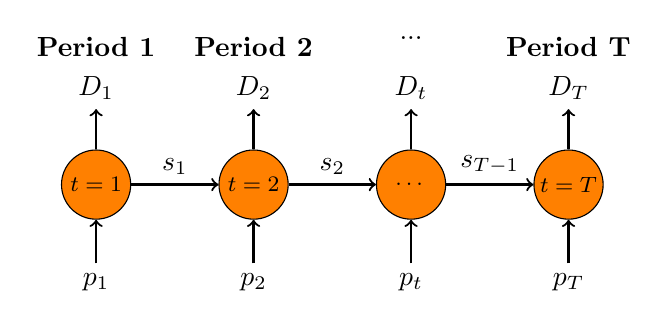
\begin{tikzpicture}[scale=1,
	node/.style={circle, fill=orange, draw, minimum size=2.5em, inner sep=1pt, font = \footnotesize}] 
		\node[below] at (0, 3) {\bf Period 1};                                                                                  
		\node[below] at (2, 3) {\bf Period 2};
		\node[below] at (4, 3) {...};
    	\node[below] at (6, 3) {\bf Period T};
    	\node[below] (11) at (0, 0) {$p_1$};                                                                                  
		\node[below] (21) at (2, 0) {$p_2$};
		\node[below] (31) at (4, 0) {$p_t$};
    	\node[below] (41) at (6, 0) {$p_T$};
    	\node[below] (12) at (0, 2.5) {$D_1$};                                                                                  
		\node[below] (22) at (2, 2.5) {$D_2$};
		\node[below] (32) at (4, 2.5) {$D_t$};
	    \node[below] (42) at (6, 2.5) {$D_T$};	    
		\node[node] (1) at (0, 1) {$t=1$};
		\node[node] (2) at (2, 1) {$t=2$};
		\node[node] (3) at (4, 1) {$\dots$};
		\node[node] (4) at (6, 1) {$t=T$};
		\draw[->, thick] (1) -- node[above] {$s_1$} (2);
		\draw[->, thick] (2) -- node[above] {$s_2$} (3) ;
		\draw[->, thick] (3) -- node[above] {$s_{T-1}$}(4);
		\draw[->, thick] (11) -- (1);
		\draw[->, thick] (21) -- (2);
		\draw[->, thick] (31) -- (3);
		\draw[->, thick] (41) -- (4);   
		\draw[->, thick] (1) -- (12);
		\draw[->, thick] (2) -- (22);
		\draw[->, thick] (3) -- (32);
		\draw[->, thick] (4) -- (42);                                     
	\end{tikzpicture}                    
	\caption{A schematic representation of the lot-sizing problem. Each node represents the material balance at each time period $t$.} \label{p1c1:fig:lot-sizing_diagram}		
\end{figure}

The production planning problem can be formulated as
%
\begin{flalign*}
	\mini & \sum_{t \in T} \left[C_t p_t + H s_t\right] \\
	\st 	  & p_t + s_{t-1} = D_t + s_t, \ \forall t \in T \\
	      & p_t, h_t \geq 0, \ \forall t \in T .	
\end{flalign*}
%

A few points must be considered carefully when dealing with lot-sizing problems. First, one must carefully consider boundary condition, that is what the model is deciding in time periods $t = T$ and what is the initial initial inventory (carried from $t=0$). While the former will be seen by the model as the ``end of the world'' and thus will realise that optimal inventory levels must be zero, the latter might considerable influence how much production is needed during the planning horizon $T$. These must be observed and handled accordingly. 
 


\section{The geometry of LPs - graphical method} 

Let us now focus our attention to the geometry of linear programming (LP) models. As it will become evident later one, LP models have a very peculiar geometry that is exploited by one of the most widespread methods to solve them. 

\subsection{The graphical method}

In order to create a geometric intuition, we will utilise a graphical representation of the resource allocation example (the paint factory problem). But first, recall the general LP formulation \eqref{p1c1:eq:LP_objective}--\eqref{p1c1:eq:LP_domain}, where $A$ is an $m \times n$ matrix, and $b$, $c$, and $x$ have suitable dimensions. Let $a_i$ be one of the $m$ rows of $A$. Notice each constraint $a_i^\top x \leq b_i$ defines a closed half-space, with boundary defined by a hyperplane $a_i^\top x= b_i$, $\forall i \in I = \braces{1,\dots,m} \equiv [m]$. By plotting all of these closed half-spaces we can see that their intersection will form the \emph{feasible region} of the problem, that is, the (polyhedral) set of point that satisfy all constraints $Ax \le b$. 


Figure \ref{p1c1:fig:feasible_region_plot} provides a graphical representation of the feasible region of the paint factory problem. 
%
\begin{figure}[h]
	\begin{subfigure}{0.45\textwidth}
		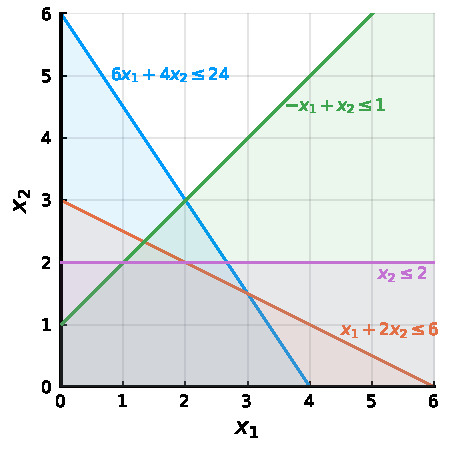
\includegraphics[scale=0.99]{./part_1/chapter_1/figures/ex2_c4.pdf}	
		\caption{}
	\end{subfigure}
	\begin{subfigure}{0.45\textwidth}
		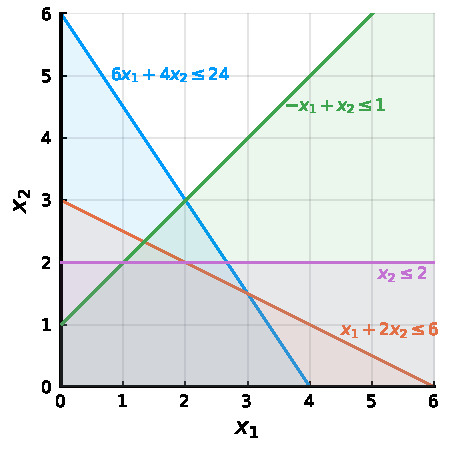
\includegraphics[scale=0.99]{./part_1/chapter_1/figures/ex2_c4.pdf}
		\caption{}		
	\end{subfigure}
	\caption{The feasible region of the paint factory problem, represented as the intersection of the four closed-half spaces formed by each of the constraints. Notice how the feasible region is a polyhedral set in $\reals^2$, as there are two decision variables ($x_1$ and $x_2$).} \label{p1c1:fig:feasible_region_plot}	
\end{figure}
%

We can use this visual representation to find the optimal solution for the problem, that is, the point $(x_1,x_2)$ within the feasible set such that the objective function value is minimal. For that, we must consider how the objective function $z = c^\top x$ can be represented in the $(x_1, x_2)$-plane. Notice that the objective function forms a hyperplane in $(x_1, x_2, z) \subset \reals^3$, of which we can plot level curves (i.e., projections) onto the $(x_1, x_2)$-plane. Figure \ref{p1c1:fig:level_curves_a} shows the plotting of three level curves, for $z= 5, 10$, and $15$. 
%
\begin{figure}
	\begin{subfigure}{0.45\textwidth}
		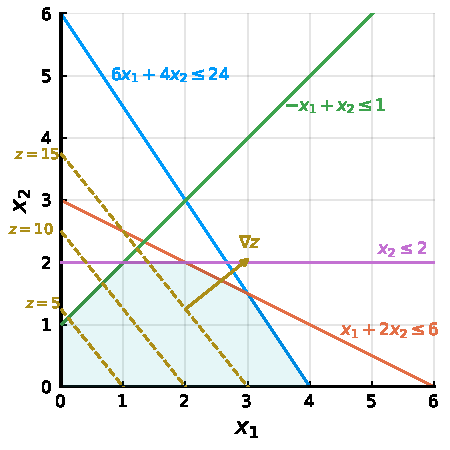
\includegraphics[scale=0.99]{part_1/chapter_1/figures/ex2_c5.pdf}  
		\caption{} \label{p1c1:fig:level_curves_a}	
	\end{subfigure}
	\begin{subfigure}{0.45\textwidth}
		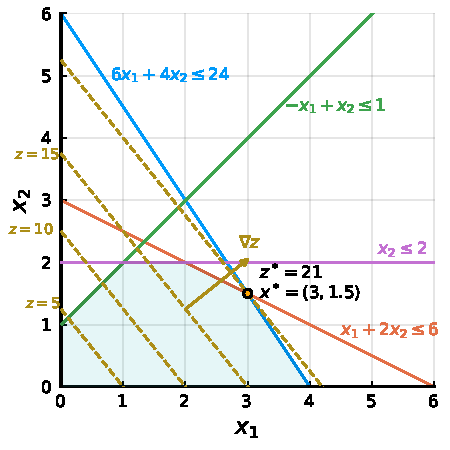
\includegraphics[scale=0.99]{part_1/chapter_1/figures/ex2_complete.pdf}
		\caption{} \label{p1c1:fig:level_curves_b}	 
	\end{subfigure}
	\caption{Graphical representation of some of the level curves of the objective function $z = 5x_1 + 4x_2$. Notice that the constant gradient vector $\nabla z = (5,4)^\top$ points to the direction in which the level curves increase in value. The optimal point is represented by $x^*=(3, 1.5)^\top$ with the furthermost level curve being that associated with the value $z^* = 21$}	
\end{figure}
%
This observation provides us with a simple graphical method to find the optimal solution of linear problems. One must simply sweep the feasible region in the direction of the gradient $\nabla z=[\frac{\partial z}{\partial x_1},\frac{\partial z}{\partial x_2}]^\top=[5,4]^\top$ (or opposite to it, if minimising) until one last point (or edge) or contact remains, meaning that the whole of the feasible region is behind that furthermost level curve. Figure \ref{p1c1:fig:level_curves_b} illustrates the processing of finding the optimal solution for the paint factory problem.

The graphical method is important because it allows to observe several key features that are going to be used later on when we define a method that can search for optimal solutions for LP problems. The first is related to the notion of active or inactive constraints. We say that a constraint is \emph{active} if, at the optimum, the constraint is satisfied as an equality. For example, the constraints $6x_1 + 4x_2 \leq 24$ and $x_1 + 2x_2 \leq 6$ are active at the optimum $x^* = (3, 1.5)$, since $6(3) + 4(1.5) = 24$ and $3 + 2(1.5) = 6$. An active constraint indicates that the resource (or requirement) represented by that constraint is being fully depleted (or minimally satisfied). 

Analogously, \emph{inactive constraint} are constraints that are satisfied as strict inequalities at the optimum. For example, the constraint $-x_1 + x_2 \leq 1$ is inactive at the optimum, as $-(3) + 1.5 < 1$. In this case, an inactive constraint represents a resource (or requirement) that is not fully depleted (or is over satisfied).


\subsection{Geometrical properties of LPs}

One striking feature concerning the geometry of LPs that becomes evident when we analyse the graphical method is that the number of candidate solutions is not infinite, but yet, only \emph{a finite set} of points are potential candidates for optimal solution. This is because the process of sweeping in the direction of the gradient will, in general, lead to a unique solution that must lie on a vertex of the polyhedral feasible set. The only exceptions are either when the gradient $\nabla z$ happens to be perpendicular to a facet of the polyhedral set (and in the direction of the sweeping) or in case the sweeping direction is not bounded by some of the facets of the polyhedral set. These exceptional cases will be discussed in more detail later on, but the observation still holds.

In the graphical example (i.e., in $\reals^2$), notice how making $n = 2$ constraints active out of $m = 4$ constraints \emph{forms a vertex}. However, not all vertices are feasible. This allows us to devise a mechanism to describe vertices (by activating $n$ of the $m$ constraints) which we could exhaustively test and select the best. The issue however, is that the number of candidates increases \emph{exponentially} with the number of constraints and variables	 of the problem, which would quickly become computationally infeasible. As we will see, it turns out that this search idea can be made considerably efficient and the underlying framework of the \emph{simplex method}, however there are worst-case settings where the method does need to consider every single vertex.

The simplex method exploits the above idea to \emph{heuristically} search for solutions by selecting $n$ constraints to be active from the $m$ constraints available. Starting from an initial selection of constraints to be active, it selects one inactive constraint to activate and one to deactivate in a way that improvement in the objective function can observed while feasibility is maintained. This process repeats until no improvement can be observed. When such is the case, the \emph{geometry} of the problem guarantees \emph{(global) optimality}. In the following chapters we will concentrate on defining algebraic objects that we will use to develop the simplex method.



		
	\part{Nonlinear optimisation}
		
	\chapter{Introduction}
	\section{What is optimisation?}

An optimisation is one of these words that has many meanings, depending on the context you take as a reference. In the context of this course, optimisation refers to \emph{mathematical optimisation}, which is a discipline of applied mathematics.

In mathematical optimisation, we build upon concepts and techniques from calculus, analysis, linear algebra, and other domains of mathematics to develop methods that allow us finding values for variables within a given domain that maximise (or minimise) the value of a function. In specific, we are trying to solve the following general problem:
%
\begin{align}
    \min &f(x) \label{eq:opt_prob} \\
    \text{s.t.}   &x \in X. \nonumber
\end{align}
%
%where $x \in \reals^n$ is a vector of $n$ \emph{variables}, $f:\mathbb{R}^n \mapsto \reals$ is a \emph{function} to be optimised (minimised) and $X \subseteq \reals^n$ is a \emph{domain} containing acceptable values for $x$.

In a general sense, these problems can be solved by employing the following strategy:
%
\begin{enumerate}
    \item Analysing properties of functions under specific domains and deriving the conditions that must be satisfied such that a point $x$ is a candidate optimal point.
    \item Applying numerical methods that iteratively searches for points satisfying these conditions. 
\end{enumerate}
%
This idea is central in several domains of knowledge, and very often are defined under area-specific nomenclature. Fields such as economics, engineering, statistics, machine learning and, perhaps more broadly, operations research, are intensive users and developers of optimisation theory and applications. 

\subsection{Mathematical programming and optimisation}

Operations research and mathematical optimisation are somewhat intertwined, as they both were born around a similar circumstance. %(Include something on the history of OR)

I like to separate \emph{mathematical programming} from (mathematical) \emph{optimisation}. Mathematical programming is a modelling paradigm, in which we rely on (very powerful, I might add) analogies to model \emph{real-world} problems. In that, we look at a given decision problem considering that
%
\begin{itemize}
    \item \emph{variables} represent \emph{decisions}, as in a business decision or a course of action. Examples include setting the parameter of (e.g., prediction) model, production systems layouts, geometries of structures, topologies of networks, and so forth; 
    \item \emph{domain} represents business rules or \emph{constraints}, representing logic relations, design or engineering limitations, requirements, and such; 
    \item function is an \emph{objective function} that provides a measure of solution quality.  
\end{itemize}
%    
With these in mind, we can represent the decision problem as a \emph{mathematical programming model} of the form of \eqref{eq:opt_prob} that can be solved using \emph{optimisation} methods. From now on, we will refer to this specific class of models as mathematical optimisation models, or optimisation models for short. We will also use the term to \emph{solve the problem} to refer to the task of finding optimal solutions to optimisation models.

This course is mostly focused on the optimisation techniques employed to find optimal solutions for these models. As we will see, depending on the nature of the functions $f$ and $g$ that are used to formulate the model, some methods might be more or less appropriate. Further complicating the issue, for models of a given nature, there might be alternative algorithms that can be employed and with no generalised consense whether one method is generally better performing than another.

\subsection{Types of mathematical optimisation models}

In general, the simpler the assumptions on the parts forming the optimisation model, the more efficient are the methods to solve such problems. 

Let us define some additional notation that we will use from now on. Consider a model in the general form
%
\begin{align*}
	\mini & f(x) \\
	\st   & g_i(x) \leq 0, i = 1, \dots, m \\
	      & h_i(x) = 0, i = 1, \dots, l \\
	      & x \in X,  
\end{align*}
%
where $f: \reals^n \mapsto \reals$ is the objective function, $g:\reals^m \mapsto \reals^m$ is a collection of $m$ inequality constraints and $h: \reals^n \mapsto \reals^l$ is a collection of $l$ equality constraints.

{\bf Remark:} in fact, every inequality constraint can be represented by an equality constraint by making $h_i(x) = g_i(x) + x_{n+1}$ and augmenting the decision variable vector $x \in \reals^n$ to include the slack variable $x_{n+1}$. However, since these constraints are of very different nature, we will explicitly represent both whenever necessary.

The most general types of models are the following. We also use this as an opportunity to define some (admittedly confusing) nomenclature from the field of operations research that we will be using in these notes.
%
\begin{enumerate}
    \item \emph{Unconstrained models:} in these, the set $X = \reals^n$ and $m=l=0$. These are prominent in, e.g., machine learning and statistics applications, where $f$ represents a measure of model fitness or prediction error.  
    \item \emph{Linear programming (LP):} presumes linear objective function. $f(x) = c^\top x$ and constraints $g$ and $h$ affine, i.e., of the form $a_i^\top x - b_i$, with $a_i \in \reals^n$ and $b \in \reals$. Normally, $X = \braces{x \in \reals^n \mid x_j \geq 0, j = 1,\dots, n}$ enforce that decision variables are constrained to be the nonnegative orthant.
    \item \emph{Nonlinear programming (NLP):} some or all of the functions $f$, $g$, and $h$ are nonlinear.
    \item \emph{Mixed-integer (linear) programming (MIP):} consists of an LP in which some (or all) of the variables are constrained to be integers. In other words, $X \subseteq \reals^k \times \integers^{n-k}$. Very frequently, the integer variables are binary terms, i.e., $x_i \in \braces {0,1}$, for $i = 1,\dots, n-k$ and are meant to represent true-or-false or yes-or-no conditions.
    \item \emph{Mixed-integer nonlinear programming (MINLP):} are the intersection of MIPs and NLPs.  
\end{enumerate}

{\bf Remark:} notice that we use the vector notation $c^\top x = \sum_{j \in J} c_j x_j$, with $J = \braces{1,\dots,N}$. This is just a convenience for keeping the notation compact. 


\section{Examples of applications}


We now discuss a few examples to illustrate the nature of the problems to which we will develop solution methods and their applicability to real-world contexts. 

\subsection{Resource allocation and portfolio optimisation} \label{sec:resource_allocation}

In a general sense, any mathematical optimisation model is an instantiation of the \emph{resource allocation problem}. A resource allocation problem consists of how to design an optimal allocation of resources to tasks, such that a given outcome is optimised. 

Classical examples typically include production planning settings, in which raw materials or labour resources are inputted into a system and a collection of products, a production plan, results from this allocation. The objective is to find the best production plan, that is, a plan with the maximum profit or minimum cost. Resource allocation problems can also appear in a less obvious setting, where the resources can be the capacity of transmission lines in an energy generation planning setting, for example.

Let $i \in I = \braces{1,\dots, M}$ be a collection of resources and $j \in J = \braces{1,\dots,N}$ be a collection of products. Suppose that, to produce one unit of product $j$, a quantity $a_{ij}$ of resource $i$ is required. Assume that the total availability of resource $i$ is $b_i$ and that the return per unit of product $j$ is $c_j$.

Let $x_j$ be the decision variable representing total of product $j$ produced. The resource allocation problem can be modelled as
%
\begin{align}
	\maxi \ & \sum_{j \in J} c_j x_j \label{ex1:obj} \\
	\st & \sum_{j \in J}a_{ij} x_j \leq b_i, \ \forall i \in I \label{ex1:const1} \\
	& x_j \geq 0, \ \forall j \in J. \label{ex1:const2}
\end{align} 
%
Equation \eqref{ex1:obj} represents the objective function, in which we maximise the total return obtained from a given production plan. Equation \eqref{ex1:const1} quantify the resource requirements for a given production plan and enforce that such a requirement does not exceed the resource availability. Finally, constraint \eqref{ex1:const2} defines the domain of the decision variables.

Notice that, as posed, the resource allocation problem is linear. This is perhaps the most basic, and also most diffused setting for optimisation models for which very reliable and mature technology is available. In this course, we will concentrate on methods that can solve variants of this model in which the objective function and/or the constraints are required to include nonlinear terms. 

One classic variant of resource allocation that include nonlinear terms is the \emph{portfolio optimisation problem}. In this, we assume that a collection of assets $j \in J = \braces{1,\dots, N}$ are available for investment. In this case, capital is the single (actual) resource to be considered. Each asset has random return $R_j$, with an expected value $\mathbb{E}[R_j] = \mu_j$. Also, the covariance between two assets $i,j \in J$ is given by $\sigma_{ij} = \mathbb{E}[(R_i - \mu_i)(R_j - \mu_j)]$, which can be denoted as the covariance matrix 
%
\begin{align*}
	\Sigma = \begin{bmatrix}
		\sigma_{11} & \dots & \sigma_{1N} \\ 
		\vdots      & \ddots & \vdots \\
		\sigma_{N1}  & \dots & \sigma_{NN}
	\end{bmatrix}
\end{align*}
%
Markowitz (1952) proposed using $x^\top\Sigma x$ as a risk measure that captures the variability in the return of the assets. Given the above, the optimisation model that provides the investment portfolio with the least risk, given a minimum requirement $\epsilon$ in terms of expected returns is given by
%
\begin{align}
	\mini \ &  x^\top\Sigma x \label{ex2:obj} \\
	\st & \mu^\top x  \geq \epsilon \label{ex2:const1}\\
	& 0 \leq x_j \leq 1, \ \forall j \in J. \label{ex2:const2}
\end{align} 
%
Objective function \eqref{ex2:obj} represents the portfolio risk to be minimised, while constraint \eqref{ex2:const1} enforces that the expected return must be at least $\epsilon$. Notice that $\epsilon$ can be seen as a resource that has to be (at least) completely depleted, if one wants to do a parallel with the resource allocation structure discussed early. Constraint \eqref{ex2:const2} defined the domain of the decision variables. Notice how the problem is posed in a scaled form, where $x_j \in [0,1]$ represents a percentage of a hypothetical available capital for investment.

In this example, the problem is nonlinear due to the quadratic nature of the objective function $x^\top\Sigma x = \sum_{i,j \in J} \sigma_{ij}x_ix_j$. As we will see later on, there are efficient methods that can be employed to solve quadratic problems like this.


\subsection{The pooling problem: refinery operations planning}

The \emph{pooling problem} is another example of a resource allocation problem that naturally presents nonlinear constraints. In this case, the production depends on \emph{mixing operations}, known as pooling, to obtain certain product specification for a given property.

As an illustration, suppose that products $j \in J = \braces{1,\dots,N}$ are produced by mixing byproducts $i \in I_j \subseteq I = \braces{1,\dots,M}$. Assume that the qualities of byproducts $q_i$ are known and that there is no reaction between byproducts. Each product is required to have a property value $q_j$ within an acceptable range $[\underline{q}_j, \overline{q}_j]$ to be classified as product $j$. In this case, mass and property balances are calculated as
%
\begin{align}
	& x_j  = \sum_{i \in I_j}{x_i}, \ \forall j \in J \\
	& q_j = \frac{\sum_{i \in I_j}q_ix_i}{x_j}, \ \forall j \in J \label{ex3:const2}.
\end{align}
%
These can then incorporated into the resource allocation problem accordingly. One key aspect associated with pooling problem formulations is that the property balances represented by \eqref{ex3:const2} define \emph{nonconvex} feasibility regions. As we will see later, convexity is a powerful property that allows for developing efficient solution methods and its absence typically compromises computational performance and tractability in general.

  
\subsection{Robust optimisation}

Robust optimisation is a subarea of mathematical programming concerned with models that support decision-making under \emph{uncertainty}. In specific, the idea is to devise a formulation mechanism that can guarantee feasibility of the optimal solution in face of variability, ultimately taking a risk-averse standpoint. 

Consider the resource allocation problem from Section \ref{sec:resource_allocation}. Now, suppose that the parameters $\tilde{a}_i \in \reals^N $ associated with a given constraint $i \in I = \braces{1,\dots,M}$ are uncertain with a unknown probability distribution. The resource allocation problem can then be formulated as
%
\begin{align*}
	\maxi \ &  c^\top x  \\
	\st & \tilde{a}_{i}^\top x \leq b_i, \ \forall i \in I  \\
	& x_j \geq 0, \ \forall j \in J. 
\end{align*} 
%
Let us assume that the only information available are observations $\hat{a}_i$, from which we can estimate a nominal value $\overline{a}_i$. This is illustrated in Figure \ref{fig:random_observations}, in which 100 random observations are generated for $\tilde{a_i} = [\tilde{a}_{i1}, \tilde{a}_{i2}]$ with $\tilde{a}_{i1} \sim \text{Normal}(10,2)$ and $\tilde{a}_{i2} \sim \text{Normal}(5,3)$ for a single constraint $i \in I$. The nominal values are assumed to have coordinates given by the average values used in the Normal distributions. 
%
\begin{figure}[h]
	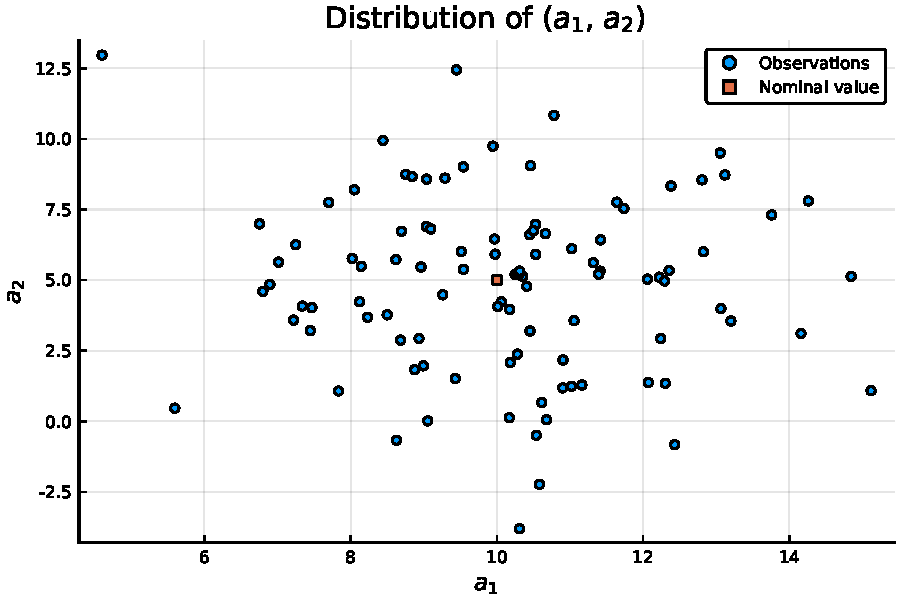
\includegraphics[width=0.8\textwidth]{part_2/chapter_1/figures/data_no_ellipsoid.pdf}
	\caption{One hundred random realisations for $\tilde{a}_i$.} \label{fig:random_observations}
\end{figure}
%
Our objective is to develop a model that incorporates a given level of protection in terms of feasibility guarantees. That is, we would like to develop a model that provides solutions that are guaranteed to remain feasible if the realisation of $\tilde{a}_i$ falls within an \emph{uncertainty set} $\epsilon_i$ of size controlled by the parameter $\Gamma_i$. The idea is that the bigger the uncertainty set $\epsilon_i$, the more robust is the solution, which typically comes at the expense of accepting solutions with expected worse performance.

The tractability of robust optimisation models depends on the geometry of the uncertainty set employed. Let us assume in what follows that 
%
\begin{align}
	\epsilon_i = \braces{\overline{a}_i + P_iu \mid ||u||_2 \leq \Gamma_i} \label{eq:ellipsoid}
\end{align}
%
is an ellipsoid with the characteristic matrix $P_i$ (i.e., its eigenvalues show how the ellipsoid extends in every direction from $\overline{a}_i$) and $\Gamma_i$ employs a scaling of the ellipsoid size.

{\bf Remark:} an alternative (perhaps more frequent) characterisation of an ellipsoid $\epsilon \subset \reals^n$ centred at $\overline{x}$ is given by $\epsilon = \braces{x \in \reals^n \mid (x - \overline{x})^\top A(x - \overline{x}) = 1}$. By making $A = P^{-2}$, we recover the representation in \eqref{eq:ellipsoid}.

We can now formulate the \emph{robust counterpart}, which consists of a risk-averse version of the original resource allocation problem. In that, we try to anticipate the worst possible outcome and make decisions that are both optimal and guarantee feasibility in this worst-case sense. This standpoint translates into the following optimisation model.
%
\begin{align}
	\maxi \ &  c^\top x \nonumber \\
	\st & \maxi_{a_{i} \in \epsilon_i}\braces{a_i^\top x} \leq b_i, \ \forall i \in I \label{ex3:robust_const}\\
	& x_j \geq 0, \forall j \in J. \nonumber
\end{align}
%
Notice how the constraint \eqref{ex3:robust_const} has an embedded optimisation problem, turning into a \emph{bi-level optimisation} problem. This highlights the issue associated with tractability, since solving the whole problem strongly depends on deriving tractable equivalent reformulations.

Assuming that the uncertainty set $\epsilon_i$ is an ellipsoid, the following result holds.
%
\begin{align}
	\max_{a_{i} \in \epsilon_i}\braces{a_i^\top x}  & = \overline{a}_i^\top x + \max_u\braces{u^\top P_i x : ||u||_2 \leq \Gamma_i} \label{eq:robust_set1}\\
	& = \overline{a}_i^\top x + \Gamma_i||P_i x||_2. \label{eq:robust_set2}
\end{align}
%
In \eqref{eq:robust_set1}, we recast the inner problem in terms of the ellipsoidal uncertainty set, ultimately meaning that we recast the inner maximisation problem in terms of variable $u$. Since the only constraint is $||u||_2 \leq \Gamma_i$, in \eqref{eq:robust_set2} we can derive a closed form for the inner optimisation problem.

With the closed form derived in \eqref{eq:robust_set2}, we can reformulate the original bi-level problem as a tractable single-level problem of the following form
%
\begin{align}
	\maxi \ &  c^\top x \nonumber \\
	\st & \overline{a}_i^\top x + \Gamma_i||P_i x||_2 \leq b_i, \ \forall i \in I \label{eq:robust_counter1}\\
	& x_j \geq 0, \ \forall j \in J. \nonumber
\end{align} 
%
Notice how the term $\Gamma_i||P_i^\top x||_2$ creates a buffer for constraint \eqref{eq:robust_counter1}, ultimately preventing the complete depletion of the resource. Clearly, this will lead to a suboptimal solution when compared to the original deterministic at the expense of providing protection against deviations in coefficients $a_i$. This difference is often referred to as the \emph{price of robustness}.

In Figure \ref{fig:ellipsoids}, we show the ellipsoidal sets for two levels of $\Gamma_i$ for a single constraint $i$. We define 
%
\begin{align}
	\epsilon_i = \braces{\begin{bmatrix} 10 \\ 5 \end{bmatrix} + \begin{bmatrix} 2 & 0 \\ 0 & 3 \end{bmatrix} \begin{bmatrix} u_1 \\ u_2 \end{bmatrix}}
\end{align}
%
using the average and standard deviation of the original distributions that generated the observations. We plot the ellipsoids for $\Gamma_1 = 1$ and $\Gamma_2 = 1.5$, illustrating how the protection level increases as $\Gamma$ increases. This can be inferred since the uncertainty set covers more of the observations and the formulation is such that feasibility is guaranteed for any observation within the uncertainty set. 
%
\begin{figure}
	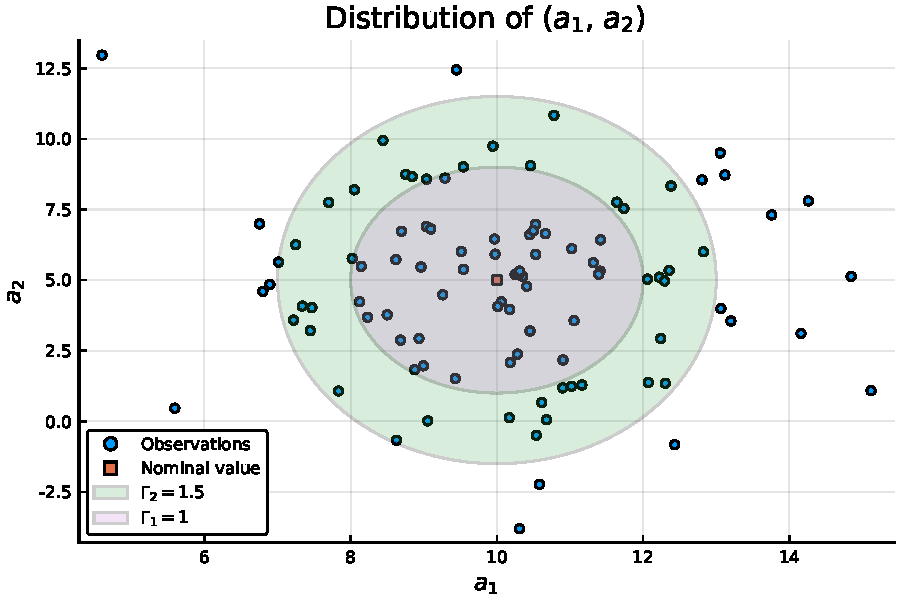
\includegraphics[width=0.8\textwidth]{part_2/chapter_1/figures/data_with_ellipsoid.pdf}
	\caption{One hundred random realisations for $\tilde{a}_i$.} \label{fig:ellipsoids}
\end{figure}
%


\subsection{Classification: support-vector machines}

This is an example in which the resource allocation structure within the optimisation model is not as obvious. Suppose we are given a data set $D \in \reals^{n}$ with $|D| = N + M$ that can be divided into two disjunct sets $I^- = \braces{x_1, \dots, x_N}$ and $I^+ = \braces{x_1,\dots, x_M}$. 

Each element in $D$ is an observation of a given set of $n$ features with values represented by a $x \in \reals^n$ that has been classified as belonging to set $I^-$ and $I^+$. Because of the availability of labelled data, classification is said to be ane xample of supervised learning in the field of machine learning. 

Figure \ref{fig:classified_observations} illustrates this situation for $n = 2$, in which the orange dots represent points classified as belonging to $I^-$ (negative observations) and the blue dots represent points classified as belonging to $I^+$ (positive observations).

\begin{figure}
    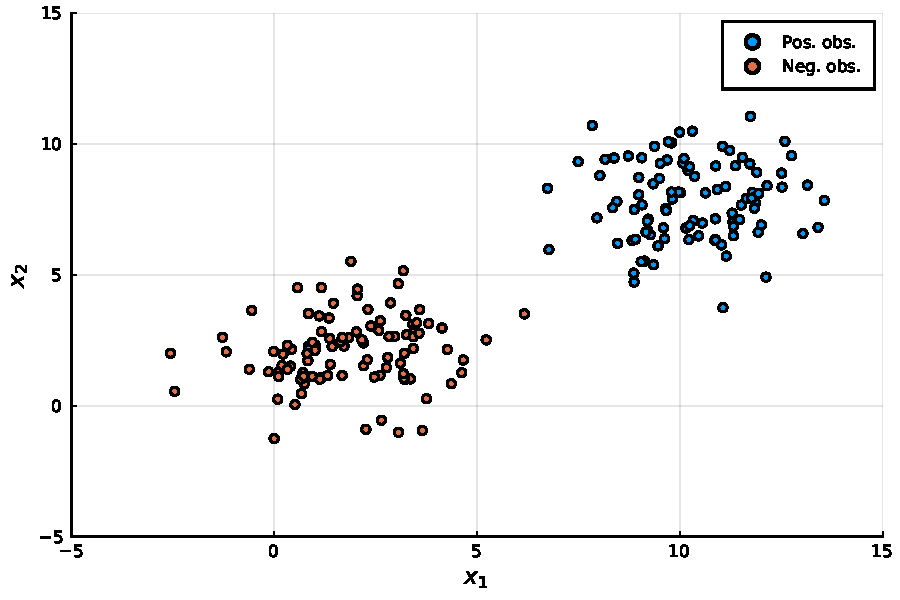
\includegraphics[width=0.8\textwidth]{part_2/chapter_1/figures/classes_no_classifier.pdf}
    \caption{Two hundred observations for $x_i$ classified to belong to $I^-$ (orange) or $I^+$ (blue).}        
    \label{fig:classified_observations}
\end{figure}

Our task is to obtain a function $f:\reals^n \mapsto \reals$ from a given family of functions that is capable to, given an observed set of features $\hat{x}$, classify whether it belongs to $I^-$ or $I^+$. In other words, we want to calibrate $f$ such that
%
\begin{align}
	f(x_i) < 0, \ \forall x_i \in I^-, \text{ and } f(x_i) > 0, \ \forall x_i \in I^+.  
\end{align}
%
This function would then act as a classifier that could be employed to any new observation $\hat{x}$ made. If $f$ is presumed to be an affine function of the form $f(x) = a^\top x - b$, then we obtain a \emph{linear classifier}. 

Our objective is to obtain $a \in \reals^n$ and $b \in \reals$ such that misclassification error is minimised. Let us define the error measure as
%
\begin{align*}
& e^-(x_i \in I^-; a, b) := 
    \begin{cases} 0, \text{ if } a^\top x_i - b \leq 0, \\
        a^\top x_i - b, \text{ if } a^\top x_i - b > 0.
    \end{cases} \\
& e^+(x_i \in I^+; a, b) := 
    \begin{cases} 0, \text{ if } a^\top x_i - b \geq 0, \\
        b -  a^\top x_i, \text{ if } a^\top x_i - b < 0.
    \end{cases}                   
\end{align*}
%
Using this error measure, we can define constraints that capture deviation on each measure by means of nonnegative slack variables. Let $u_i \geq 0$ for $i = 1, \dots, N$ and $v_i \geq 0$ for $i = 1,\dots, M$ be slack variables that measure the \emph{misclassification error} for $x_i \in I^-$ and $x_i \in I^+$, respectively.

The optimisation problem that finds optimal parameters $a$ and $b$ can be stated as
%
\begin{align}
	\mini \ & \sum_{i=1}^M u_i + \sum_{i=1}^N v_i \label{ex4:obj}\\
	\st & a^\top x_i - b - u_i \leq 0, i = 1, \dots, M \label{ex4:const1} \\
    & a^\top x_i - b + v_i \geq 0, i = 1,\dots,N \label{ex4:const2} \\
    & ||a||_2 = 1 \label{ex4:const3} \\
    & u_i \geq 0, i = 1, \dots, N \\
    & v_i \geq 0, i = 1, \dots, M \\
    & a \in \reals^n, b \in \reals. \label{ex4:end}   
\end{align} 
%
The objective function \eqref{ex4:obj} accumulates the total misclassification error. Constraint \eqref{ex4:const1} allows for capturing the misclassification error for each $x_i \in I^-$. Notice that $u_i = \max\braces{0, a^\top x_i -b} = e^-(x_i \in I^-; a, b)$. Likewise, constraint \eqref{ex4:const2} guarantees that $v_i = e^+(x_i \in I^+; a, b)$.
To avoid trivial solutions in which $(a,b) = (0, 0)$, the normalisation constraint $|| a ||_2 = 1$ is imposed in constraint \eqref{ex4:const3}, which turns the model nonlinear.

Solving the model \eqref{ex4:obj}--\eqref{ex4:end} provides optimal $(a,b)$ which translates into the classifier represented as the green line in Figure \ref{fig:observations_with_classifier}.

\begin{figure}[h]
    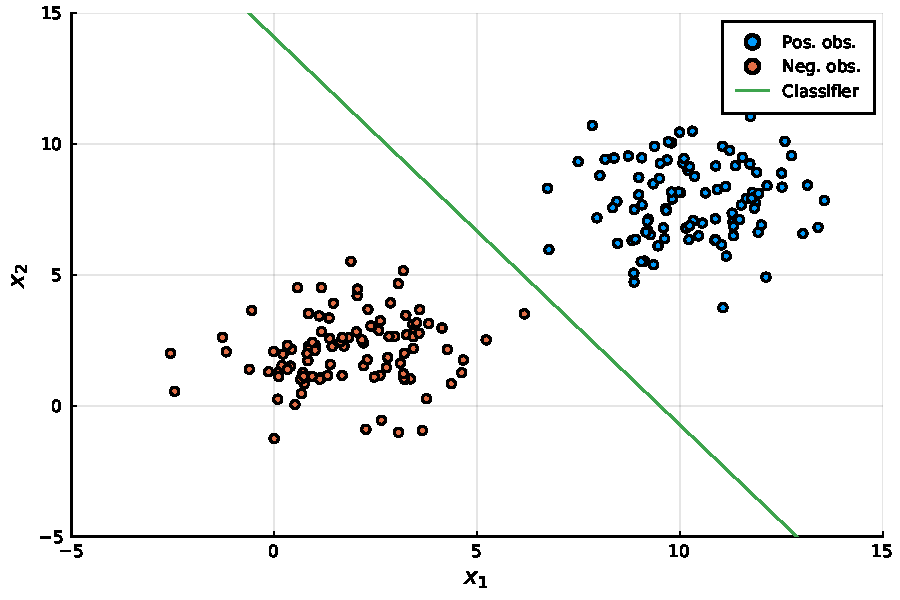
\includegraphics[width=0.8\textwidth]{part_2/chapter_1/figures/classes_with_classifier.pdf}
    \caption{Two hundred observations for $x_i$ classified to belong to $I^-$ (orange) or $I^+$ (blue) with a classifier (green).}        
    \label{fig:observations_with_classifier}
\end{figure}
 
A variant referred to as \emph{robust classifier} penalises not only the the misclassification error, but also the observations within a given slab $S = \braces{x \in \reals^n \mid -1 \leq a^\top x - b \leq 1}$. Notice that, being the two lines defined by $f^-(x) : a^\top x - b = -1$ and $f^+(x) : a^\top x - b = +1$, the distance between the two hyperplanes is given by $\frac{2}{||a||_2}$. 

Accordingly, we redefine our error measures as follows. 
%
\begin{align*}
	& e^-(x_i \in I^-; a, b) := 
	    \begin{cases} 0, \text{ if } a^\top x_i - b \leq -1, \\
	        |a^\top x_i - b|, \text{ if } a^\top x_i - b > -1.
	    \end{cases} \\
	& e^+(x_i \in I^+; a, b) := 
	    \begin{cases} 0, \text{ if } a^\top x_i - b \geq 1, \\
	        |b -  a^\top x_i|, \text{ if } a^\top x_i - b < 1.
	    \end{cases}                   
\end{align*}
%
By doing so, a penalty is applied not only to those points that were misclassified but also to those points correctly classified that happen to be inside the slab $S$. To define an optimal robust classifier, one must trade off the size of the slab, which is inversely proportional to $||a||$, and the total of observations that fall in the slab $S$. The formulation for the robust classifier then becomes
%
\begin{align}
	\mini \ & \sum_{i=1}^M u_i + \sum_{i=1}^N v_i + \gamma||a||_2^2 \label{ex5:obj}\\
	\st & a^\top x_i - b - u_i \leq -1, \ i = 1,\dots,M \label{ex5:const1} \\
	    & a^\top x_i - b + v_i \geq 1, \ i = 1,\dots,N \label{ex5:const2} \\
	    & u_i \geq 0, i = 1, \dots, N \\
	    & v_i \geq 0, i = 1, \dots, M \\
	    & a \in \reals^n, b \in \reals.
\end{align} 
%  
In objective function \eqref{ex5:obj}, the errors accumulated in variables $u_i$, $i=1,\dots,N$ and $v_i$, $i = 1,\dots,M$ and the squared norm $||a||_2^2$ are considered simultaneously. The term $\gamma$ is a scalar used to impose an emphasis on minimising the norm $||a||_2$ and incentivising a larger slab $S$ (recall that the slab is large for smaller $||a||_2$). The squared norm  $||a||_2^2$ is considered instead as a means to recover differentiability, as the norm  $||a||_2$ is not differentiable. Later on, we will see how beneficial it is for optimisation methods to be able to assume differentiability. Moreover, note how in constraints \eqref{ex5:const1} and \eqref{ex5:const2} $u$ and $v$ also accumulate penalties for correctly classified $x_i$ that happen to be between the slab $S$, that is, that have term $a^\top x - b$ larger/ smaller than -1/ +1. Figure \ref{fig:observations_with_rob_classifier} shows a robust classifier an arbitrary value of $\gamma$.

\begin{figure}[H]
    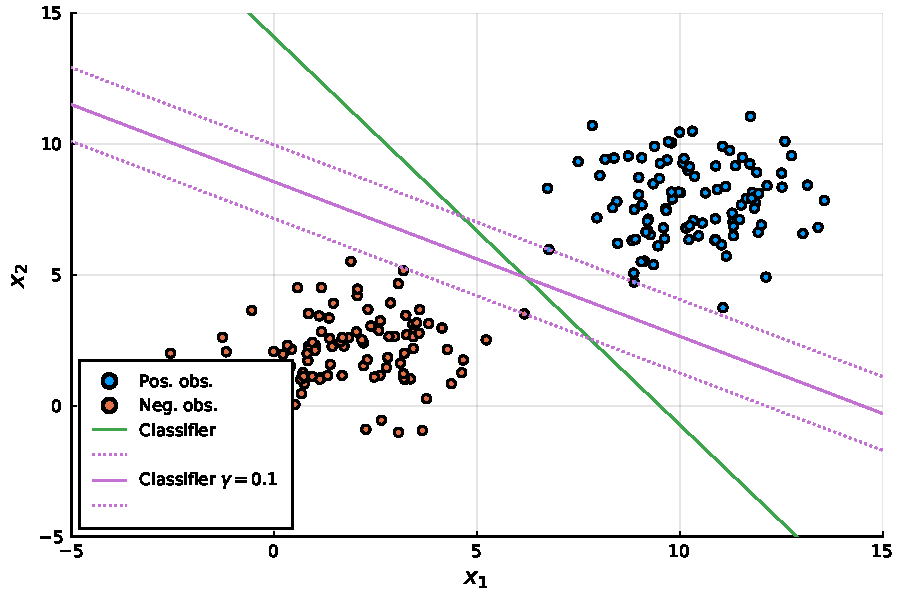
\includegraphics[width=0.8\textwidth]{part_2/chapter_1/figures/classes_with_robust_classifier.pdf}
    \caption{Two hundred observations for $x_i$ classified to belong to $I^-$ (orange) or $I^+$ (blue).}        
    \label{fig:observations_with_rob_classifier}
\end{figure}


{\bf Remark:} robust classifiers are known in the machine learning literature as \emph{support vector machines}, where the support vectors are the observations that support the slab. 

	
	\chapter{Convex sets}
	

\section{Convexity and optimisation}

\emph{Convexity} is perhaps the most important property that the elements forming an optimisation problem can present. Paraphrasing Tyrrell Rockafellar:

\begin{quote}
... in fact, the great watershed in optimization isn't between linearity and nonlinearity, but convexity and nonconvexity.
\end{quote}

The importance of convexity will become clear later in the course. In a nutshell, the existence of convexity allows us to infer global properties of a solution (i.e., that holds for all of its domain) by considering exclusively local information (such as gradients, for example). This is critical in the context of optimisation, since most of the methods we know to perform well in practice are designed to find solutions that satisfy local optimality conditions. Once convexity is attested, one can then guarantee that these local solutions are in fact globally optimal without exhaustively exploring the solution space. 

For a problem of the form
% 
\begin{align*}
    (P) :~ \mini & f(x) \\
    \st & x \in X
\end{align*}
%
to be convex, we need to verify whether $f$ is a \emph{convex function} and $X$ is a \emph{convex set}. If both statements hold true, we can conclude that $P$ is a \emph{convex problem}. We start looking into how to identify convex sets, since we can use the convexity of sets to infer the convexity of functions.


\section{Identifying convexity of sets}
 
Before we formally define convex sets, let us first look at the idea of \emph{combinations}. For that, let $S \subseteq \reals^n$ be a set and $x_j \in S$ for $j=1,\dots,k$ be a collection of vectors (i.e., $n$-dimensional ``points'') belonging to $S$. Then, we have that:
%
\begin{itemize} 
	\item A \emph{linear combination} of $x_j$ for $j=1,\dots, k$ is the set 
%
	\begin{align}
		\braces{x \in \reals^n : \sum_{j=1}^k \lambda_jx_j, \ \lambda_j \in \reals \text{ for } j=1,\dots, k}.
	\end{align}
%
	\item An \emph{affine combination} is a linear combination, with the additional constraint that $\sum_{j=1}^k \lambda_j = 1$. That is,
%
	\begin{align}
		\braces{x \in \reals^n : \sum_{j=1}^k \lambda_jx_j, \ \sum_{j=1}^k \lambda_j = 1, \ \lambda_j \in \reals \text{ for } j=1, \dots, k}.
	\end{align}
%
	\item A \emph{conic combination} is a linear combination with the additional condition that $\lambda_j \geq 0$ for $j = 1,\dots,k$.
%
	\begin{align}
		\braces{x \in \reals^n : \sum_{j=1}^k \lambda_jx_j, \ \lambda_j \geq 0 \text{ for } j=1,\dots,k}.
	\end{align}
%
	\item And finally, a \emph{convex combination} is the intersection between an affine and a conic combinations, implying that $\lambda_j \in [0,1]$.  
%
	\begin{align}
		\braces{x \in \reals^n : \sum_{j=1}^k \lambda_jx_j, \ \sum_{j=1}^k \lambda_j = 1, \ \lambda_j \geq 0 \text{ for } j=1,\dots,k}.
	\end{align}
% 
\end{itemize}

We say that a set is convex if it contains all points formed by the convex combination of any pair of points in this set. This is equivalent to saying that the set contains the line segment between any two points belonging to the set. 

\begin{definition}[Convex sets] \label{def:convex_sets}
	A set $S \subseteq \reals^n$ is said to be convex if $\overline{x} = \sum_{j=1}^k \lambda_jx_j$ belongs to $S$, where $\sum_{j=1}^k \lambda_j = 1$, $\lambda_j \geq 0$ and $x_j \in S$ for $j=1,\dots, k$.
\end{definition}

Definition \ref{def:convex_sets} is useful as it allows for showing that some set operations preserve convexity. 

\subsection{Convexity-preserving set operations}

\begin{lemma}[Convexity-preserving operations] \label{lem:convex_operations}
	Let $S_1$ and $S_2$ be convex sets in $\reals^n$. Then, the sets resulting from the following operations are also convex.
	\begin{enumerate}
		\item {Intersection:} $S = S_1 \cap S_2$;
		\item {Minkowski addition:} $S = S_1 + S_2 = \braces{x_1 + x_2 : x_1 \in S_1, x_2 \in S_2}$;
		\item {Minkowski\hspace{-1pt} difference:}\hspace{-2pt} $S = S_1 - S_2 = \braces{x_1 - x_2 : x_1 \in S_1, x_2 \in S_2}$;
		\item {Affine transformation:} $S = \braces{Ax + b : x \in S_1}$.
	\end{enumerate}
\end{lemma}

Figures \ref{fig:mink_sum} and \ref{fig:intersection} illustrate the concept behind some of these set operations. Showing that the sets resulting from the operations in Lemma \ref{lem:convex_operations} are convex typically entails showing that convex combinations of elements in the resulting set $S$ also belong to $S_1$ and $S_2$.

\begin{figure}
	\centering
    	\begin{tikzpicture}
%    		\draw[help lines] (-6,-3) grid (6,3);
    		\node (picture) at (0,0) {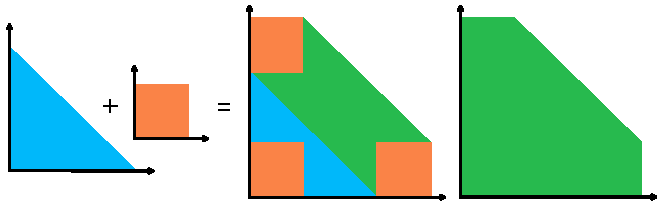
\includegraphics{part_2/chapter_2/figures/mink_sum}};
    		\node (A) at (-5, -0.5) {$S_1$};
    		\node (B) at (-2.9, -0.1) {$S_2$};
    		\node (C) at (-1, 1) {$S_2$};		
    		\node (D) at (-1, -1.1) {$S_2$};
    		\node (E) at (1.2, -1.1) {$S_2$};
    		\node (F) at (3, -0.5) {$S$};
    		\node (G) at (-1.1, -0.15) {$S_1$};
    	\end{tikzpicture}
		\caption{Minkowski sum of two convex sets.}\label{fig:mink_sum}
\end{figure}

%
\begin{figure}
	\centering
    \begin{tikzpicture}
%    		\draw[help lines] (-2,-2) grid (2,2);
    		\node (picture) at (0,0) {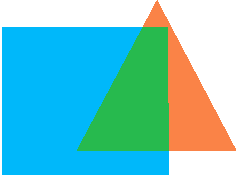
\includegraphics{part_2/chapter_2/figures/intersection.pdf}};
    		\node (A) at (-1, -0.15) {$S_1$};
    		\node (B) at (1.2, -0.5) {$S_2$};
    		\node (C) at (0.2, -0.8) {$S_1 \cap S_2$};
    \end{tikzpicture}
    
    \caption{Intersection of two convex sets.} \label{fig:intersection}
\end{figure}
%

\subsection{Examples of convex sets}

There are several familiar sets that are known to be convex. Having the knowledge that these sets are convex is useful as a building block for determining the convexity of more complicated sets.

Some important examples of convex sets include:
\begin{itemize}
	\item Them empty set $\emptyset$, any singleton $\{\overline{x}\}$ and the whole space $\reals^n$; 
	\item halfspaces: $S = \braces{x : p^\top x \leq \alpha} \subset \reals^n$;
	\item hyperplanes: $H = \braces{x : p^\top x = \alpha} \subset \reals^n$, where $p \neq 0^n$ is a normal vector and $\alpha\in \reals$ is a scalar. Notice that $H$ can be equivalently represented as $H = \braces{x \in \reals^n: p^\top(x - \overline{x}) = 0}$ for $\overline{x} \in H$;
	\item polyhedral sets: $P = \braces{x : Ax \leq b} \subset \reals^n$, where $A\in \reals^{m\times n}$ and $b \in \reals^n$;
	\item norm-induced sets (balls): $B = \braces{x : ||x - \overline{x}|| \leq \alpha} \subseteq \reals^n$, where $|| \cdot ||$ is any norm and $\alpha$ a scalar;
	\item norm cones: $C =\braces{(x,\alpha) \in \reals^{n+1}: ||x|| \leq \alpha} $;
\end{itemize} 

For example, let us consider the polyhedral set $P = \braces{x \in \reals^n : Ax \leq b} \subset \reals^n$ with $A$ being a $m \times n$ matrix. Notice that $S$ is the intersection of a collection of half-spaces $H_i = \braces{x \in \reals^n : a_i^\top x \leq b_i}$, where $a_i$ are vectors from the rows of the matrix $A$ and $b_i$ are the components of the column vector $b$. We know that $H_i$ are convex sets, thus $P = \cap_{i=1}^m H_i$ is also convex, as the intersection of sets is a convexity-preserving set operation.


\subsubsection{Hyperplanes and halfspaces}

Hyperplanes and halfspaces will play a central role in the developments we will see in our course. Therefore, let us take a moment and discuss some important aspects related these convex sets. First, notice that, geometrically, a hyperplane $H \subset \reals^n$ can be interpreted as the set of points with a \emph{constant} inner product to a given vector $p \in \reals^n$, while $\overline{x}$ determines the offset of the hyperplane from the origin. That is,
	\begin{equation*}
		H = \braces{x : p^\top(x - \overline{x}) = 0} \equiv \overline{x} + p^{\perp},
	\end{equation*}
	where $p^\perp$ is the orthogonal complement of $p$, i.e., the set of vectors orthogonal to $p$, which is given by $\braces{x \in \reals^n : p^\top x = 0}$.
	
	\begin{figure}[H]
	    \begin{tikzpicture}
%    		\draw[help lines] (-2,-2) grid (2,2);
    		\node (picture) at (0,0) {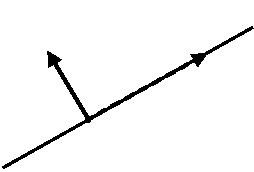
\includegraphics{part_2/chapter_2/figures/hyperplane.pdf}};
    		\node (p) at (-1.3, 0.8) {$p$};
    		\node (xbar) at (-0.6, -0.8) {$\overline{x}$};
    		\node (H) at (2, 0.5) {$H$};
		\end{tikzpicture}
		\caption{A hyperplane $H = \braces{x \in \reals^n: p^\top(x - \overline{x}) = 0}$ with normal vector $p$ displaced to $\overline{x}$.}
	\end{figure}
	
	Analogously, a halfspaces can be represented as $S = \braces{x \in \reals^n : p^\top(x - \overline{x}) \le 0}$ where $p^\top \overline{x} = \alpha$ is the hyperplane that forms the boundary of the halfspace. This definition suggests a simple geometrical interpretation: the halfspace $S$ consists of $\overline{x}$ plus any vector with an obtuse or right angle (i.e., greater of equal to 90$^\circ$) with the outward normal vector $p$.
 
 	\begin{figure}[H]
	    \begin{tikzpicture}
%    		\draw[help lines] (-2,-2) grid (2,2);
    		\node (picture) at (0,0) {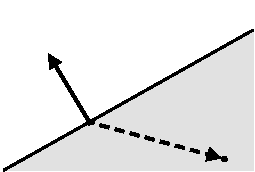
\includegraphics{part_2/chapter_2/figures/halfspace.pdf}};
    		\node (p) at (-1.3, 0.75) {$p$};
    		\node (xbar) at (-0.6, -0.9) {$\overline{x}$};
    		\node (x) at (1.9, -1.3) {$x$};
    		\node (H) at (1.7, 0.3) {$S$};
		\end{tikzpicture}
		\caption{A halfspace $S = \braces{x \in \reals^n : p^\top(x - \overline{x}) \le 0}$ defined by the same hyperplane $H$. Notice how the vectors $p$ (or $p - \overline{x}$, which is fundamentally the same vector but translated to $\overline{x}$) and $x - \overline{x}$ form angles greater or equal than $90^\circ$.}
	\end{figure}
	
	\begin{figure}[H]
    \begin{tikzpicture}
%    		\draw[help lines] (-2,-2) grid (2,2);
    		\node (picture) at (0,0) {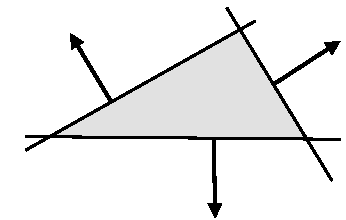
\includegraphics{part_2/chapter_2/figures/polyhedral_set.pdf}};
    		\node (P) at (0.75, 0.25) {$P$};
    		\node (a1) at (-1.6, 1.4) {$a_1$};
    		\node (a2) at (1, -1.8) {$a_2$};    		
    		\node (a2) at (2.8, 1.3) {$a_3$};
    \end{tikzpicture}
    \caption{A polyhedron $P$ formed by the intersection of three halfspace. Each hyperplane $H_i = \braces{x \in \reals^n : a_i^\top x \leq b_i}$, for $i = 1,2,3$, has a normal vector $a_i$, and has an offset from the origin $b_i$ (which cannot be seen once project on a 2-dimensional plane as in the picture).} \label{fig:polyhedral_set}
\end{figure}

\subsubsection{Norm balls and norm cones}

An Euclidean ball (or simply ball) of radius $\epsilon$ in $\reals^n$ has the form
%
\begin{equation*}
	B(\overline{x}, r) = \braces{x \in \reals^n : || x - \overline{x}||_2 \le \epsilon} \equiv \braces{x \in \reals^n : (x - \overline{x})^\top (x - \overline{x}) \le \epsilon^2}
\end{equation*}
%
As one might suspect, balls are convex, which can be proved by noting that
%
\begin{align*}
	||\lambda x_1 + (1 - \lambda) x_2 - \overline{x}||_2  & = ||\lambda (x_1 - \overline{x}) + (1 - \lambda) (x_2 - \overline{x})||_2 \\
	& \le \lambda ||x_1 - \overline{x}||_2 + + (1 - \lambda) ||x_2 - \overline{x}||_2 \le \epsilon.
\end{align*}
%
Notice that between the first and the second line, we use the triangle inequality, which states that $||x + y|| \le ||x|| + ||y||$ for any two vectors $x$ and $y$ and any norm (including the Euclidean norm). 

Euclidean balls are a special case of norm balls, which are defined as $B(\overline{x}, r) = \braces{x \in \reals^n : || x - \overline{x}|| \le \epsilon}$ where $||\ \cdot \ ||$ is any norm on $\reals^n$. 

A related set is the norm cone, defined as $C(x, \alpha) = \braces{(x,\alpha) \in \reals^{n+1} : ||x|| \le \alpha}$, where $\alpha$ is a scalar. For example, the second-order cone (also known as the ice cream cone or Lorentz cone) is the norm cone for the Euclidean norm.

\begin{remark} 
	Norm induced sets (balls or cones) are convex for any norm $||x||_p = \left(\sum_{i=1}^n x_i^p\right)^{\frac{1}{p}}$ for $x \in \reals^n$ and $p \geq 1$.
\end{remark}


\section{Convex hulls} 

A \emph{convex hull} of a set $S$, denoted $\conv(S)$ is the set formed by all convex combinations of all points in $S$. As the name suggests, $\conv(S)$ is a convex set, regardless of $S$ being or not convex. 

Another interpretation for $\conv(S)$ is to think of it as the tightest enveloping (convex) set that contains $S$. Notice that, if $S$ is convex, then $S = \conv(S)$.  Formally, convex hulls are defined as follows.

\begin{definition}[Convex hull of a set]\label{def: convex_hull}
	Let $S \subseteq \reals^n$ be an arbitrary set. The convex hull of $S$, denoted by $\conv(S)$, is the collection of all convex combinations of $S$. That is, for $x_j \in S$, with $j = 1,\dots, k$, $x \in \conv(S)$ if and only if 
	%
	\begin{equation*}
		x = \sum_{j=1}^k \lambda_jx_j : \sum_{j=1}^k \lambda_j = 1, \ \lambda_j \geq 0, \text{ for } j = 1,\dots,k.
	\end{equation*}                       
	%
\end{definition}
%

From Definition \ref{def: convex_hull}, one can show that the convex hull $\conv(S)$ can also be defined as the intersection of all convex sets containing $S$. Perhaps the easiest way to visualise this is to think of the infinitely many half-space containing $S$ and their intersection, which can only be $S$. Figure \ref{fig:convex_hull} illustrates the convex hull $\conv(S)$ of an nonconvex set $S$.
%
\begin{figure}[H]
%
\includegraphics[width=0.3\textwidth]{Figures/convex_hull.pdf}
	\begin{tikzpicture}
%    		\draw[help lines] (-3,-2) grid (3,2);
    		\node (picture) at (0,0) {
\includegraphics{part_2/chapter_2/figures/convex_hull.pdf}};
    		\node (A) at (-1.5, 0) {$S$};
    		\node (B) at (0.3, 0.5) {$\conv(S)$};
    \end{tikzpicture}
\caption{Example of an arbitrary set $S$ (in solid blue) and its convex hull $\conv(S)$ (combined blue and grey areas).} \label{fig:convex_hull}
\end{figure}
%
The notion of convex hulls is a powerful tool in optimisation. One important application is using $\conv(S)$ to obtain approximations for a nonconvex $S$ that can be exploited to solve an optimisation problem with constraint set defined by $S$. This is the underpinning technique in many important optimisation methods for such as branch-and-bound-based methods for nonconvex problems and decomposition methods (i.e., methods that solve large problems by breaking it into smaller parts that are presumably easier to solve).  

In specific, let us consider the convex hull of a finite collection of discrete points. Some of these sets are so important in optimisation that they have their own names. 
%
\begin{definition}
Let $S = \braces{x_1, \dots, x_{n+1}} \subset \reals^n$. Then $\conv(S)$ is called a \emph{polytope}. If $x_1,\dots,x_{n+1}$ are affinely independent (i.e., $x_2 - x_1, \dots ,x_{n+1} - x_1$ are linearly independent) then $\conv(S)$ is called a \emph{simplex} with vertices $x_1,\dots,x_{n+1}$.
\end{definition}
%


%\subsection{The Carath\'eodory theorem*}
%
%
%The \emph{Carath\'eodory theorem} is an important result associated with simplexes. It states that if $x \in \conv(S) \subset \reals^n$, then there exists a simplex composed by $x_j \in S$ for $j = 1, \dots, n+1$ that contains $x$. Formally, the theorem is posed as follows.
%%
%\begin{theorem}[Carath\'eodory theorem]
%Let $S \subseteq \reals^n$. If $x \in \conv(S)$, then $x \in \conv(x_1, \dots, x_{n+1})$ for some $x_j \in S$ where $j = 1,\dots, n+1$.        
%\end{theorem}   
%
%%% Consider including a proof for the Caratheodory theorem, for the sake of completeness.
%
%
%More specifically, any point $x \in \conv(S)$ can be expressed as
%%
%\begin{equation*}
%	x = \sum_{j=1}^{n+1} \lambda_jx_j : \sum_{j=1}^{n+1} \lambda_j = 1, \ \lambda_j \geq 0, \text{ for } j = 1,\dots,{n+1},
%\end{equation*}
%%
%for a given collection of points $x_j$, with $j = 1, \dots, n+1$ forming a simplex. Figure \ref{fig:caratheodory} illustrates this result.
%%
%\begin{figure}[h]
%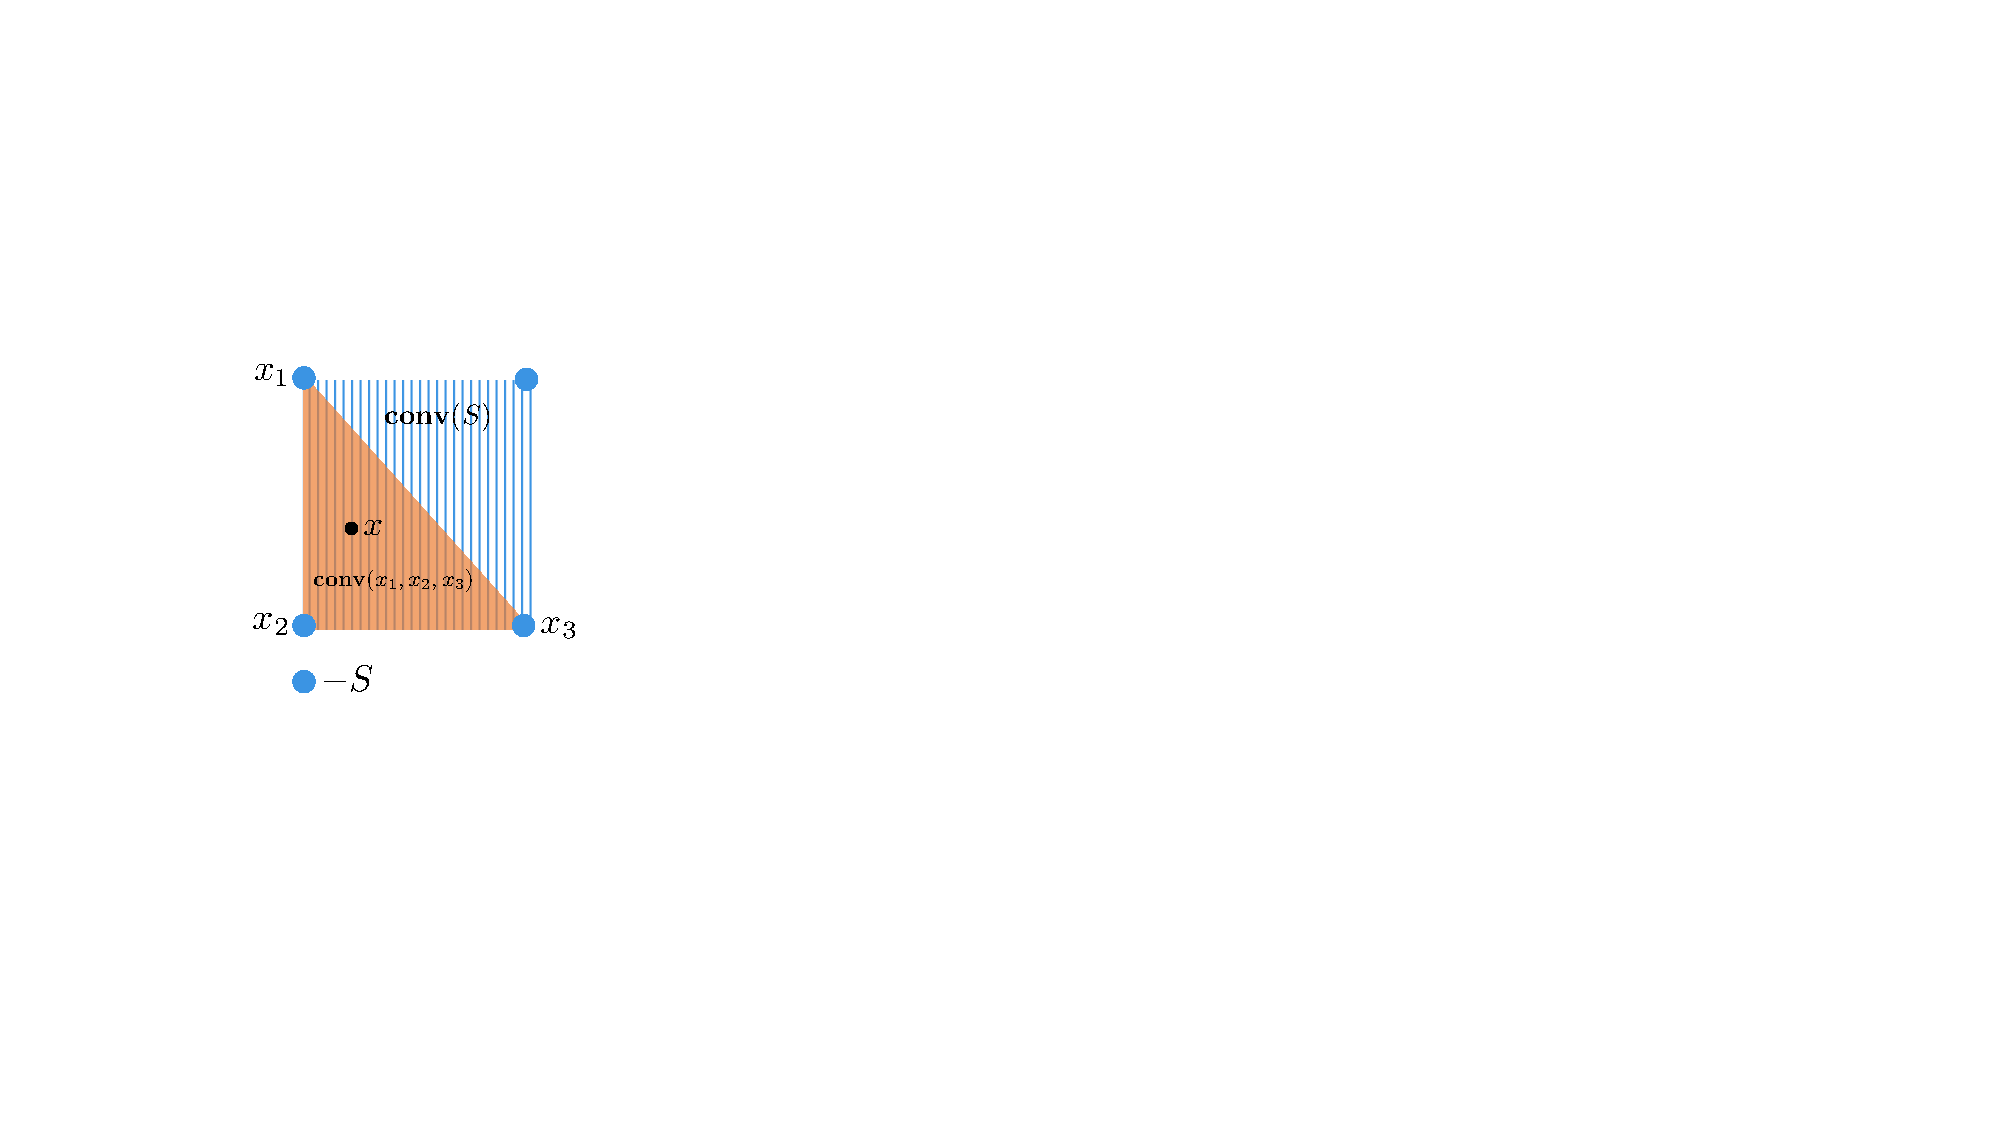
\includegraphics[width=0.3\textwidth]{Figures/caratheodory.pdf}
%\caption{Example of an arbitrary set $S$ (blue dots) and its convex hull $\conv(S)$ (light blue). Notice that $x$ can be represented as the convex combination of $x_j$ for $j=1,2,3$ for $n=2$.} \label{fig:caratheodory}
%\end{figure} 


\section{Closure and interior of sets}

Many of the set-related results we will see in this course depends on the characteristics of the set itself. Often, assuming properties such as closedness or compactness considerably ease technical derivations. 


\subsection{Closure, interior and boundary of a set}


Let us define some properties that will be useful in this course. For that, we will use an $\epsilon$-neighbourhood of $x \in \reals^n$ (which is a norm ball of radius $\epsilon$ centred in $x$) defined as
%
\begin{align*}
    N_\epsilon(x) = \braces{y : ||y - x|| < \epsilon}.
\end{align*}
%
Let $S \subseteq \reals^n$ be an arbitrary set. We can use $N_\epsilon$ to define the following elements related to $S$.  
\begin{enumerate}
\item \emph{Closure of $S$}: the set defined by the closure of $S$, denoted $\clo(S)$, is defined as 
%
\begin{align*}
\clo(S) = \braces{x \in \reals^n : S \cap N_\epsilon(x) \neq \emptyset \text{ for every } \epsilon > 0}. 
\end{align*}
%
Notice that the closure might contain points that do not belong to $S$. We say that a set is \emph{closed} if $S = \clo(S)$, that is, the set itself is its own closure. 
%
\item \emph{Interior of $S$}: the interior of $S$, denoted $\intr(S)$, is the set
\begin{align*}
\intr{S} = \braces{x \in S : N_\epsilon(x) \subset S \text{ for some } \epsilon > 0}.
\end{align*}
%
If $S$ is the same as its own interior, then we say that $S$ is \emph{open}. Some authors say that $S$ is solid if it has a nonempty interior (that is, $\intr(S) \neq \emptyset$. Notice that the interior of $S$ is a subset of $S$, that is $\intr(S) \subseteq S$.
%
\item \emph{Boundary of $S$}: the boundary of $S$, denoted $\bou(S)$ is the collection of points defined by
%
\begin{align*}
\bou(S) = \braces{x \in \reals^n : N_\epsilon(x) \text{ contains some } x_i \in S \text{ and some } x_j \notin S \text{ for every } \epsilon > 0}.
\end{align*}
%
We say that $S$ is bounded if exists $N_\epsilon(x)$, $x \in \reals^n$, for some $\epsilon > 0$ such that $S \subset N_\epsilon(x)$. 
\end{enumerate}

We say that a set is \emph{compact} if it is both \emph{closed} and \emph{bounded}. Compact sets appear very frequently in real-world applications of optimisation, since typically one can assume the existence of bounds for decision variables (such as nonnegativity or maximum physical bounds or, at an extreme case, smallest/ largest computational constants). Another frequent example of bounded set is the convex hull of a collection of discrete points, which is called by some authors \emph{polytopes} (effectively bounded polyhedral sets).  

Let us consider the following example. Let $S = \braces{(x_1,x_2) \in \reals^n : x_1^2 + x_2^2 \leq 1}$. Then, we have that:
\begin{enumerate}
	\item $\clo(S) = \braces{(x_1,x_2) \in \reals^n : x_1^2 + x_2^2 \leq 1}$. Since $S = \clo(S)$, $S$ is closed.
	\item $\intr(S) = \braces{(x_1,x_2) \in \reals^n : x_1^2 + x_2^2 < 1}$. 
	\item $\bou(S) = \braces{(x_1,x_2) \in \reals^n : x_1^2 + x_2^2 = 1}$. Notice that it makes $S$ bounded.
	\item $S$ is compact, since it is closed and bounded. 
\end{enumerate}

Notice that, if $S$ is closed, then $\bou(S) \subset S$. That is, its boundary is part of the set itself. Moreover, it can be shown that $\clo(S) = \bou(S) \cup S$ is the smallest closed set containing $S$. 

In case $S$ is convex, one can infer the convexity of the interior $\intr(S)$ and its closure $\clo(S)$. The following theorem summarises this result.
%
\begin{theorem}\label{thm:top_convex_comb}
Let $S \subseteq \reals^n$ be a convex set with $\intr(S) \neq \emptyset$. Let $x_1 \in \clo(S)$ and $x_2 \in \intr(S)$. Then $x = \lambda x_1 + (1 - \lambda) x_2 \in \intr(S)$ for all $\lambda \in (0,1)$.
\end{theorem}
%

% Consider including the proof for this theorem (on page 46)

Theorem \ref{thm:top_convex_comb} is useful for inferring the convexity of the elements related to $S$. We summarise the key results in the following corollary.
%
\begin{corollary} Let $S$ be a convex set with $\intr(S) \neq \emptyset$. Then
	\begin{enumerate}
		\item $\intr(S)$ is convex;
		\item $\clo(S)$ is convex;
		\item $\clo(\intr(S)) = \clo(S)$;
		\item $\intr(\clo(S)) = \intr(S)$.
	\end{enumerate}
\end{corollary}
%

% Consider including the proof for this corollary (on page 46)


\subsection{The Weierstrass theorem}


The Weierstrass theorem is a result that guarantees the existence of optimal solutions for optimisation problems. To make it more precise, let
%
\begin{align*}
	(P) :~ z = \mini\braces{f(x) : x \in S}  
\end{align*}
%
be our optimisation problem. If an optimal solution $x^*$ exists, then $f(x^*) \leq f(x)$ for all $x \in S$ and $z = f(x^*) = \min \braces{f(x) : x \in S}$. 

Notice the difference between $\mini$ (an abbreviation for minimise) and the operator $\min$. The first is meant to represent the problem of minimising the function $f$ in the domain $S$, while $\min$ is shorthand for minimum, in this case $z$, assuming that it is attainable.

It might be that an optimal solution is not attainable, but a bound can be obtained for the optimal solution value. The greatest lower bound for $z$ is its \emph{infimum} (or \emph{supremum} for maximisation problems), denoted by $\inf$. That is, if $z = \inf\braces{f(x) : x \in S}$ , then $z \leq f(x)$ for all $x \in S$ and there is no $\overline{z} > z$ such that $\overline{z} \leq f(x)$ for all $x \in S$. We might sometimes use the notation 
%
\begin{align*}
(P) :~ z = \inf\braces{f(x) : x \in S}
\end{align*}
%
to represent optimisation problems for which one cannot be sure whether an optimal solution is attainable. The Weierstrass theorem describes the situations in which those minimums (or maximums) are guaranteed to be attained, which is the case whenever $S$ is compact.
%
\begin{theorem}[Weierstrass theorem]\label{thm:weierstrass}
Let $S \neq \emptyset$ be a compact set, and let $f:S \rightarrow \reals$ be continuous on $S$. Then there exists a solution $\overline{x} \in S$ to $\mini\braces{f(x) : x \in S}$. 
\end{theorem}
%
Figure \ref{fig:Weierstrass} illustrates three examples. In the first (on the left) the domain $[a,b]$ is compact, and thus the minimum of $f$ is attained at $b$. In the other two, $[a,b)$ is open and therefore, Weierstrass theorem does not hold. In the middle example, one can obtain $\inf f$, which is not the case for the last example on the right.
%
\begin{figure}[h]
%\includegraphics[width=0.8\textwidth]{Figures/Weierstrass.pdf}
	\begin{tikzpicture}
%    		\draw[help lines] (-6,-1) grid (6,1);
    		\node (picture) at (0,0) {\includegraphics{part_2/chapter_2/figures/Weierstrass.pdf}};
    		\node (fa1) at (-5.8, 0.75) {$f(a)$};
    		\node (fb1) at (-5.8, -0.8) {$f(b)$};
 	    		\node (fa2) at (-1.8, 0.75) {$f(a)$};
    		\node (fb2) at (-1.8, -0.8) {$\inf f$};
 	    		\node (fa3) at (2.2, 0.75) {$f(a)$};
 	    		\node (a1) at (-5, -1.55) {$a$};
    		\node (b1) at (-3, -1.55) {$b$};
    		\node (a2) at (-1, -1.55) {$a$};
    		\node (b2) at (1, -1.55) {$b$};
 	    		\node (a3) at (3, -1.55) {$a$};
    \end{tikzpicture}
	\caption{Examples of attainable minimum (left) and infimum (centre) and an example where neither are attainable (right).} \label{fig:Weierstrass}
\end{figure}


\section{Separation and support of sets}
 

The concepts of \emph{separation} and \emph{support} of sets are key for establishing optimality conditions later in this course. We are interested in mechanisms that allow one to infer whether there exists hyperplanes separating points from sets (or sets from sets). We will also be interested in means to, given a point $x \notin S$, find the closest to point not belonging to $S$.

\subsection{Hyperplanes and closest points}

We start with how to identify closest points to sets. 
%
\begin{theorem}[Closest-point theorem]\label{thm:closest_point}
Let $S \neq \emptyset$ be a closed convex set in $\reals^n$ and $y \notin S$. Then, there exists a unique point $\overline{x} \in S$ with minimum distance from $y$. In addition, $\overline{x}$ is the minimising point if and only if $$(y-\overline{x})^\top(x - \overline{x}) \leq 0, \text{ for all } x\in S$$
\end{theorem}
%
Simply put, if $S$ is a closed convex set, then $\overline{x} \in S$ will be the closest point to $y \notin S$ if the vector $y - \overline{x}$ is such that if it forms an angle that is greater or equal than 90$^\circ$ with all other vectors $x - \overline{x}$ for $x \in S$. Figure \ref{fig:closest_point} illustrates this logic. 

\begin{figure}[h]
	\begin{tikzpicture}
%    	\draw[help lines] (-3,-2) grid (3,2);
		\node (picture) at (0,0) {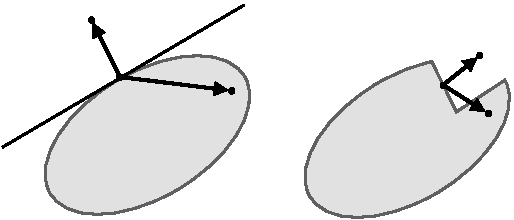
\includegraphics{part_2/chapter_2/figures/closest_point.pdf}};
		\node (y1) at (-2.8, 2) {$y$};
		\node (y2) at (4, 0.8) {$y$};
		\node (xbar1) at (-2.6, 0.4) {$\overline{x}$};
		\node (xbar2) at (2.9, 0.3) {$\overline{x}$};
		\node (x1) at (-0.4, -0.1) {$x$};    		
		\node (x2) at (3.9, -0.5) {$x$};
		\node (S) at (-2, -1) {$S$};
		\node (S) at (2, -1) {$S$};    		
    \end{tikzpicture}
	\caption{Closest-point theorem for a closed convex set (on the left). On the right, an illustration on how the absence of convexity invalidates the result.} \label{fig:closest_point}
\end{figure}

Notice that $S$ lies in the half-space $(y-\overline{x})^\top(x - \overline{x}) \leq 0$ defined by the hyperplane $p^\top(x - \overline{x}) =0$ with normal vector $p = (y - \overline{x})$. We will next revise the concepts of half-spaces and hyperplanes, since they will play a central role in the derivations in this course.  

\subsection{Halfspaces and separation}

We can use halfspaces to build the concept of separation. Let us start recalling that a hyperplane $H = \braces{x : p^\top x = \alpha}$ with normal vector $p \in \reals^n$ and $\alpha \in \reals$ defines two half-spaces $H^+ = \braces{x : p^\top x \geq \alpha}$ and $H^- = \braces{x : p^\top x \leq \alpha}$. Figure \ref{fig:hyperplane} illustrates the concept. Notice how the vector $p$ lies in the half-space $H^+$.
%
\begin{figure}
%	\includegraphics[scale=0.6]{Figures/hyperplanes.pdf}
	\begin{tikzpicture}
%    	\draw[help lines] (-2,-2) grid (2,2);
		\node (picture) at (0,0) {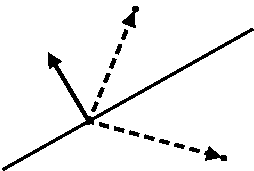
\includegraphics{part_2/chapter_2/figures/halfspaces.pdf}};
		\node (p) at (-1.4, 0.8) {$p$};
		\node (xbar) at (-0.7, -0.9) {$\overline{x}$};
		\node (H+) at (2, 1.2) {$H^{+}$};
		\node (H-) at (2, 0.5) {$H^{-}$};
	\end{tikzpicture}	
	\caption{Normal vectors, hyperplane and halfspaces} \label{fig:hyperplane}
\end{figure}
 
Any hyperplane $H$ can be defined in reference to a point $\overline{x} \in H$ by noticing that 
%
\begin{align*}
	p^\top(x - \overline{x}) = p^\top x - p^\top \overline{x} = \alpha - \alpha = 0.  
\end{align*}
%
From that, the half-spaces defined by $H$ can be equivalently stated as $H^+ = \braces{x : p^\top (x - \overline{x}) \geq 0}$ and $H^- = \braces{x : p^\top (x - \overline{x}) \leq 0}$.

We can now define the separation of convex sets. 
%
\begin{definition} \label{def:separation}
	Let $S_1$ and $S_2$ be nonempty sets in $\reals^n$. The hyperplane $H = \braces{x: p^\top x = \alpha}$ is said to \emph{separate} $S_1$ and $S_2$ if $ p^\top x \geq \alpha$ for each $x \in S_1$ and $p^\top x \leq \alpha$ for each $x \in S_2$. In addition, the following apply: 
	\begin{enumerate}
		\item {\bf Proper separation:} $S_1 \cup S_2 \not\subset H$;
		\item {\bf Strict separation:} $ p^\top x < \alpha$ for each $x \in S_1$ and $p^\top x > \alpha$ for each $x \in S_2$;
		\item {\bf Strong separation:} $ p^\top x \geq \alpha + \epsilon$ for some $\epsilon >0$ and $x \in S_1$, and $p^\top x \leq \alpha$ for each $x \in S_2$.
	\end{enumerate}
\end{definition}
%
Figure \ref{fig:separation} illustrates the three types of separation in Definition \ref{def:separation}. On the left, proper separation is illustrated, which is obtained by any hyperplane that does not contain both $S_1$ and $S_2$, but that might contain points from either or both. In the middle, sets $S_1$ and $S_2$ belong to two distinct half-spaces in a strict sense. On the right, strict separation holds with an additional margin $\epsilon > 0$, which is defined as strong separation. 
%
\begin{figure}[H]
%	\includegraphics[scale=0.8]{Figures/separations.pdf}
	\begin{tikzpicture}
%    	\draw[help lines] (-4,-2) grid (4,2);
		\node (picture) at (0,0) {\includegraphics{part_2/chapter_2/figures/separations.pdf}};
		\node (S11) at (-3.6, 0.5) {$S_1$};
		\node (S21) at (-3.15, -0.45) {$S_2$};
		\node (S12) at (-0.2, 0.5) {$S_1$};
		\node (S22) at (0.25, -0.45) {$S_2$};
		\node (S13) at (3, 0.5) {$S_1$};
		\node (S23) at (3.65, -0.45) {$S_2$};
		\node (H1) at (-2, 1.1) {$H$};		
		\node (H2) at (1.3, 1.1) {$H$};
		\node (H3) at (4.7, 1.1) {$H$};
	\end{tikzpicture}	
	\caption{Three types of separation between $S_1$ and $S_2$.} \label{fig:separation}
\end{figure}
%
A powerful yet simple result that we will use later is that, for a closed convex set $S$, there always exists a hyperplane separating $S$ and a point $y$ that does not belong to $S$.
%4
\begin{theorem}[Separation theorem]\label{thm:separation}
Let $S \neq \emptyset$ be a closed convex set in $\reals^n$ and $y \notin S$. Then, there exists a nonzero vector $p \in \reals^n$ and $\alpha \in \reals$ such that $p^\top x \leq \alpha$ for each $x \in S$ and $p^\top y > \alpha$.
\end{theorem}
%
\begin{proof}
	Theorem \ref{thm:closest_point} guarantees the existence of a unique minimising $\overline{x} \in S$ such that $(y-\overline{x})^\top(x - \overline{x}) \leq 0$ for each $x \in S$. Let $p = (y - \overline{x}) \neq 0$ and $\alpha = \overline{x}^\top(y - \overline{x}) = p^\top\overline{x}$. Then we get $p^\top x \leq \alpha$ for each $x \in S$, while $p^\top y - \alpha = (y - \overline{x})^\top(y - \overline{x}) = ||y - \overline{x}||^2 > 0$.
\end{proof}

This is the first proof we look at in these notes, and the reason for that is its importance in many of the results we will discuss further. The proof first looks at the problem of finding a minimum distance point as an optimisation problem and uses the Weierstrass theorem (our Theorem \ref{thm:closest_point} is a consequence of the Weierstrass theorem stated in Theorem \ref{thm:weierstrass}) to guarantee that such a $\overline{x}$ exists. Being a minimum distance point, we know from Theorem \ref{thm:closest_point} that $(y-\overline{x})^\top(x - \overline{x}) \leq 0$ holds. Now by defining $p$ and $\alpha$ as in the proof, one might notice that
%
\begin{align*}
	& (y-\overline{x})^\top(x - \overline{x}) \leq 0 \ \Leftrightarrow \ 
	(y-\overline{x})^\top x \leq (y - \overline{x})^\top\overline{x} \ \Leftrightarrow \ 
	p^\top x \leq p^\top\overline{x} = \alpha. 
\end{align*}
%
The inequality $p^\top y > \alpha$ is demonstrated to hold in the final part by noticing that 
%
\begin{align*}
	p^\top y - \alpha &= 
	(y - \overline{x})^\top y - \overline{x}^\top(y - \overline{x}) \\ &= 
	y^\top(y - \overline{x}) - \overline{x}^\top(y - \overline{x}) \\ & = (y - \overline{x})^\top (y - \overline{x}) = || y - \overline{x} ||^2 > 0.
\end{align*}

Theorem \ref{thm:separation} has interesting consequences. For example, one can apply it to every point in the boundary $\bou(S)$ to show that $S$ is formed by the intersection of all half-spaces containing $S$. 

Another interesting result is the existence of strong separation. If $y \notin \clo(\conv(S))$, then one can show that strong separation between $y$ and $S$ exists since there will surely be a distance $\epsilon>0$ between $y$ and $S$. 


\subsection{Farkas' theorem}

Farkas' theorem plays a central role in deriving optimality conditions. It can assume several alternative forms, which are typically referred to as Farkas' lemmas. In essence, the Farkas' theorem is used to demonstrate that a given system of linear equations has a solution if and only if a related system can be shown to have no solutions and vice-versa. 

\begin{theorem}
	Let $A$ be an $m \times n$ matrix and $c$ be an $n$-vector. Then exactly one of the following two systems has a solution:
	%
	\begin{align*}
		(1) :~ &Ax \leq 0, \ c^\top x > 0, \ x \in \reals^n\\
		(2) :~ &A^\top y = c, \ y \geq 0, \ y \in \reals^m.  
	\end{align*}
	%
\end{theorem}

\begin{proof}
	Suppose $(2)$ has a solution. Let $x$ be such that $Ax \leq 0$. Then $c^\top x = (A^\top y)^\top x = y^\top Ax \leq 0$. Hence, $(1)$ has no solution. 
	
	Next, suppose $(2)$ has no solution. Let $S = \braces{x \in \reals^n : x = A^\top y, \ y \geq 0}$. \hspace{-3pt}Notice that $S$ is closed and convex and that $c \notin S$. By Theorem \ref{thm:separation}, there exists $p \in \reals^n$ and $\alpha \in \reals$ such that $p^\top c > \alpha$ and $p^\top x \leq \alpha$ for $x \in S$. 
	
	As $0 \in S$, $\alpha \geq 0$ and $p^\top c > 0$. Also, $\alpha \geq p^\top A^\top y = y^\top Ap$ for $y \geq 0$. This implies that $Ap \leq 0$, and thus $p$ satisfies $(1)$. 
\end{proof}

The first part of the proof shows that, if we assume that system (2) has a solution, than $c^\top x > 0$ cannot hold for $y \geq 0$. The second part uses the separation theorem (Theorem \ref{thm:separation}) to show that $c$ can be seen as a point not belonging to the closed convex set $S$ for which there is a separation hyperplane and that the existence of such plane implies that system (1) must hold. The set $S$ is closed and convex since it is a conic combination of rows $a_i$, for $i=1, \dots, m$. Using the $0 \in S$, one can show that $\alpha \geq 0$. The last part uses the identity $p^\top A^\top  = (Ap)^\top$ and the fact that $(Ap)^\top y = y^\top Ap$. Notice that, since $y$ can be arbitrarily large and $\alpha$ is a constant, $y^\top Ap \leq \alpha$ can only hold if $y^\top Ap \leq 0$, requiring that $p \leq 0$ since $y \geq 0$ from the definition of $S$.

Farkas' theorem has an interesting geometrical interpretation arising from this proof, as illustrated in Figure \ref{fig:farkas}. Consider the cone $C$ formed by the rows of $A$
%
\begin{align*} 
	C = \braces{c \in \reals^n : c_j = \sum_{i=1}^m a_{ij} y_i, \ j= 1,\dots,n, \  y_i \geq 0, \ i =1,\dots, m}
\end{align*}
%
The \emph{polar cone} of $C$, denoted $C^0$, is formed by the all vectors having angles of 90$^\circ$ or more with vectors in $C$. That is, 
%
\begin{align*}
	C^0 = \braces{x : Ax \leq 0}.
\end{align*}
%
Notice that $(1)$ has a solution if the intersection between the polar cone $C^0$ and the positive ($H^+$ as defined earlier) half-space $H^+ = \braces{x \in \reals^n: c^\top x > 0}$ is not empty. If $(2)$ has a solution, as in the beginning of the proof, then $c \in C$ and the intersection $C^0 \cap H^+ = \emptyset$. Now, if $(2)$ does not have a solution, that is, $c \notin C$, then one can see that $C^0 \cap H^+$ cannot be empty, meaning that $(1)$ has a solution.  

\begin{figure}[h]
%	\includegraphics[width = 0.7\textwidth]{Figures/farkas.pdf}
	\begin{tikzpicture}
%    	\draw[help lines] (-5,-2) grid (5,2);
		\node (picture) at (0,0) {\includegraphics{part_2/chapter_2/figures/farkas.pdf}};
		\node (C01) at (-4,-0.5) {$C_0$};
		\node (C01) at (1.5,-0.7) {$C_0$};
		\node (C1) at (-1.5,-0.5) {$C$};
		\node (C2) at (4,-0.5) {$C$};
		\node (c1) at (-1.4,0) {$c$};
		\node (c2) at (2,1.7) {$c$};			
		\node (a11) at (-1.7,2) {$a_1$};
		\node (a12) at (3.8,2) {$a_1$};
		\node (a21) at (-0.8,1) {$a_2$};
		\node (a12) at (4.7,1) {$a_2$};
		\node (a31) at (-0.4,-1.3) {$a_3$};
		\node (a31) at (5.1,-1.3) {$a_3$};
	\end{tikzpicture}
	\caption{Geometrical illustration of the Farkas' theorem. On the left, system $(2)$ has a solution, while on the right, system $(1)$ has a solution} \label{fig:farkas}
\end{figure}


\subsection{Supporting hyperplanes}

There is an important connection between the existence of hyperplanes that support a whole set and optimality conditions of points. Let us first define supporting hyperplanes. 

\begin{definition}[Supporting hyperplane]
	Let $S \neq \emptyset$ be a set in $\reals^n$, and let $\overline{x} \in \bou(S)$. $H = \braces{x \in \reals^n : p^\top (x-\overline{x}) =0}$ is a supporting hyperplane of $S$ at $\overline{x}$ if either $S \subseteq H^+$ (i.e., $p^\top (x-\overline{x}) \geq 0$ for $x \in S$) or $S \subseteq H^-$.  
\end{definition}

Figure \ref{fig:support_hyperplane} illustrates the concept of supporting hyperplanes. Notice that supporting hyperplanes might not be unique, with the geometry of the set $S$ playing an important role in that matter. 

Let us define the function $f(x) = p^\top x$ with $x \in S$. One can see that the optimal solution $\overline{x}$ given by 
%
\begin{align*}
	\overline{x} = \argmax_{x \in S} f(x)
\end{align*}
%
is a point $x \in S$ for which $p$ is a supporting hyperplane. A simple geometric analogy is to think that the $f$ increases value as one moves in the direction of $p$. The constraint $x \in S$ will eventually prevent the movement further from $S$ and this last contact point is precisely $\overline{x}$. This is a useful concept for optimising problem using gradients of functions, as we will discuss later in the course.

\begin{figure}[h]
	%\includegraphics[width=0.9\textwidth]{Figures/support_hyperplane.pdf}
	\begin{tikzpicture}
%    	\draw[help lines] (-6,-2) grid (6,2);
		\node (picture) at (0,0) {\includegraphics{part_2/chapter_2/figures/support_hyperplane.pdf}};
		\node (S1) at (-4.3,-0.5) {$S$};
		\node (S2) at (-1,-0.5) {$S$};
		\node (S3) at (2.5,-0.5) {$S$};
		\node (xbar1) at (-3.6,-0.5) {$\overline{x}$};
		\node (xbar2) at (0.55,0.35) {$\overline{x}$};
		\node (p11) at (-3, -1.5) {$p$};		
		\node (p21) at (1.4, 0.75) {$p_1$};		
		\node (p22) at (1.6, 0.3) {$p_2$};
		\node (p31) at (4.3, 1.4) {$p$};
		\node (p32) at (5.05, 0.6) {$p$};
		\node (xbar31) at (3.52, 0.57) {$\overline{x}_1$};				
		\node (xbar32) at (4.25, -0.2) {$\overline{x}_2$};						
	\end{tikzpicture}
	\caption{Supporting hyperplanes for an arbitrary set. Notice how a single point might have multiple supporting planes (middle) or different points might have the same supporting hyperplane (right)} \label{fig:support_hyperplane} 
\end{figure}

One characteristic that convex sets present that will be of great importance when establishing optimality conditions is the existence of supporting hyperplanes at every boundary point.

\begin{theorem}[Support of convex sets]
	Let $S \neq \emptyset$ be a convex set in $\reals^n$, and let $\overline{x} \in \bou(S)$. Then there exists $p \neq 0$ such that $p^\top(x - \overline{x}) \leq 0$ for each $x \in \clo(S)$.
\end{theorem}

The proof follows immediately from Theorem \ref{thm:separation}, without explicitly considering a point $y \notin S$ and by noticing that $\bou(S) \subset \clo(S)$. Figure \ref{fig:support_convex} provides an illustration of the theorem. 

\begin{figure}[H]
%	\includegraphics[width=0.3\textwidth]{Figures/support_convex.pdf}
	\begin{tikzpicture}
%    	\draw[help lines] (-2,-2) grid (2,2);
		\node (picture) at (0,0) {\includegraphics{part_2/chapter_2/figures/support_convex.pdf}};
		\node (S) at (0.25,-0.5) {$S$};
		\node (S) at (-1,1.6) {$p$};
		\node (S) at (1.6, -0.1) {$\overline{x}$};
	\end{tikzpicture}
	\caption{Supporting hyperplanes for convex sets. Notice how every boundary point has at least one supporting hyperplane} \label{fig:support_convex}
\end{figure}


	
\end{document} 